%!TEX root=../../main.tex

\section{Results}
\todo{Rename Section???}



\subsection{The frameworks during setup and benchmark}
We would like to raise some issues we encountered first while installing and configuring and second while running the different frameworks.

\begin{enumerate}
	\item During setup and benchmark of Gemini, we encountered several bugs in the cloned repository. These include non zero-terminated strings or even missing return statements.

	The errors rendered the code as-is unable to perform calculations, forcing us to fork the repository and modify the source code. Our changes can be found in one of our repositories\footnote{\url{https://github.com/jasc7636/GeminiGraph}}.

	\item Furthermore, we would like to address the setup of Hadoop for Giraph. It requires multiple edits in \texttt{xml} files that aren't easily automized. This makes the setup rather time consuming, especially if reconfiguration is needed later on.
	\item In order for Giraph to run, several Java tasks (the Hadoop infrastructure) have to be constantly running in the background. While we don't expect this to have a significant performance impact on other tasks, it is still suboptimal.
	%\item The Hadoop distributed file system (HDFS) ran us into disk space problems on multiple occasions. First, unless configured otherwise, the standard implementation replicates all data three times, distributed over all participating nodes. Second, deleting files on the HDFS does not immediately free up disk space because the files are moved to a \emph{recycling bin}-like location.

	\item
\end{enumerate}


On a plus side, setup of the frameworks Polymer and Ligra was straight forward and did not require any special treatment.





%!TEX root=../../main.tex


\subsection{Single-source Shortest-paths}
For the results of our SSSP runs, we first analyze the single-node and distributed performances separately before comparing the two.

\subsubsection{Single-node}
Beginning with the single-node performance, \autoref{fig:singleNodeSSSP} shows the average calculation and execution times for SSSP on the different frameworks.

Because we did not see the perfomance going down when increasing thread counts on Galois, we always refer to Galois with 96 threads in this section (including the figures). 
For a more detailed analysis of Galois' behaviour with different thread counts, see \autoref{sec:galois_speedup}. 




TODO // Hier fehlt noch Giraph, daher noch keine vollständige Auswertung.
\begin{figure}
	\begin{subfigure}{0.3\textwidth}
		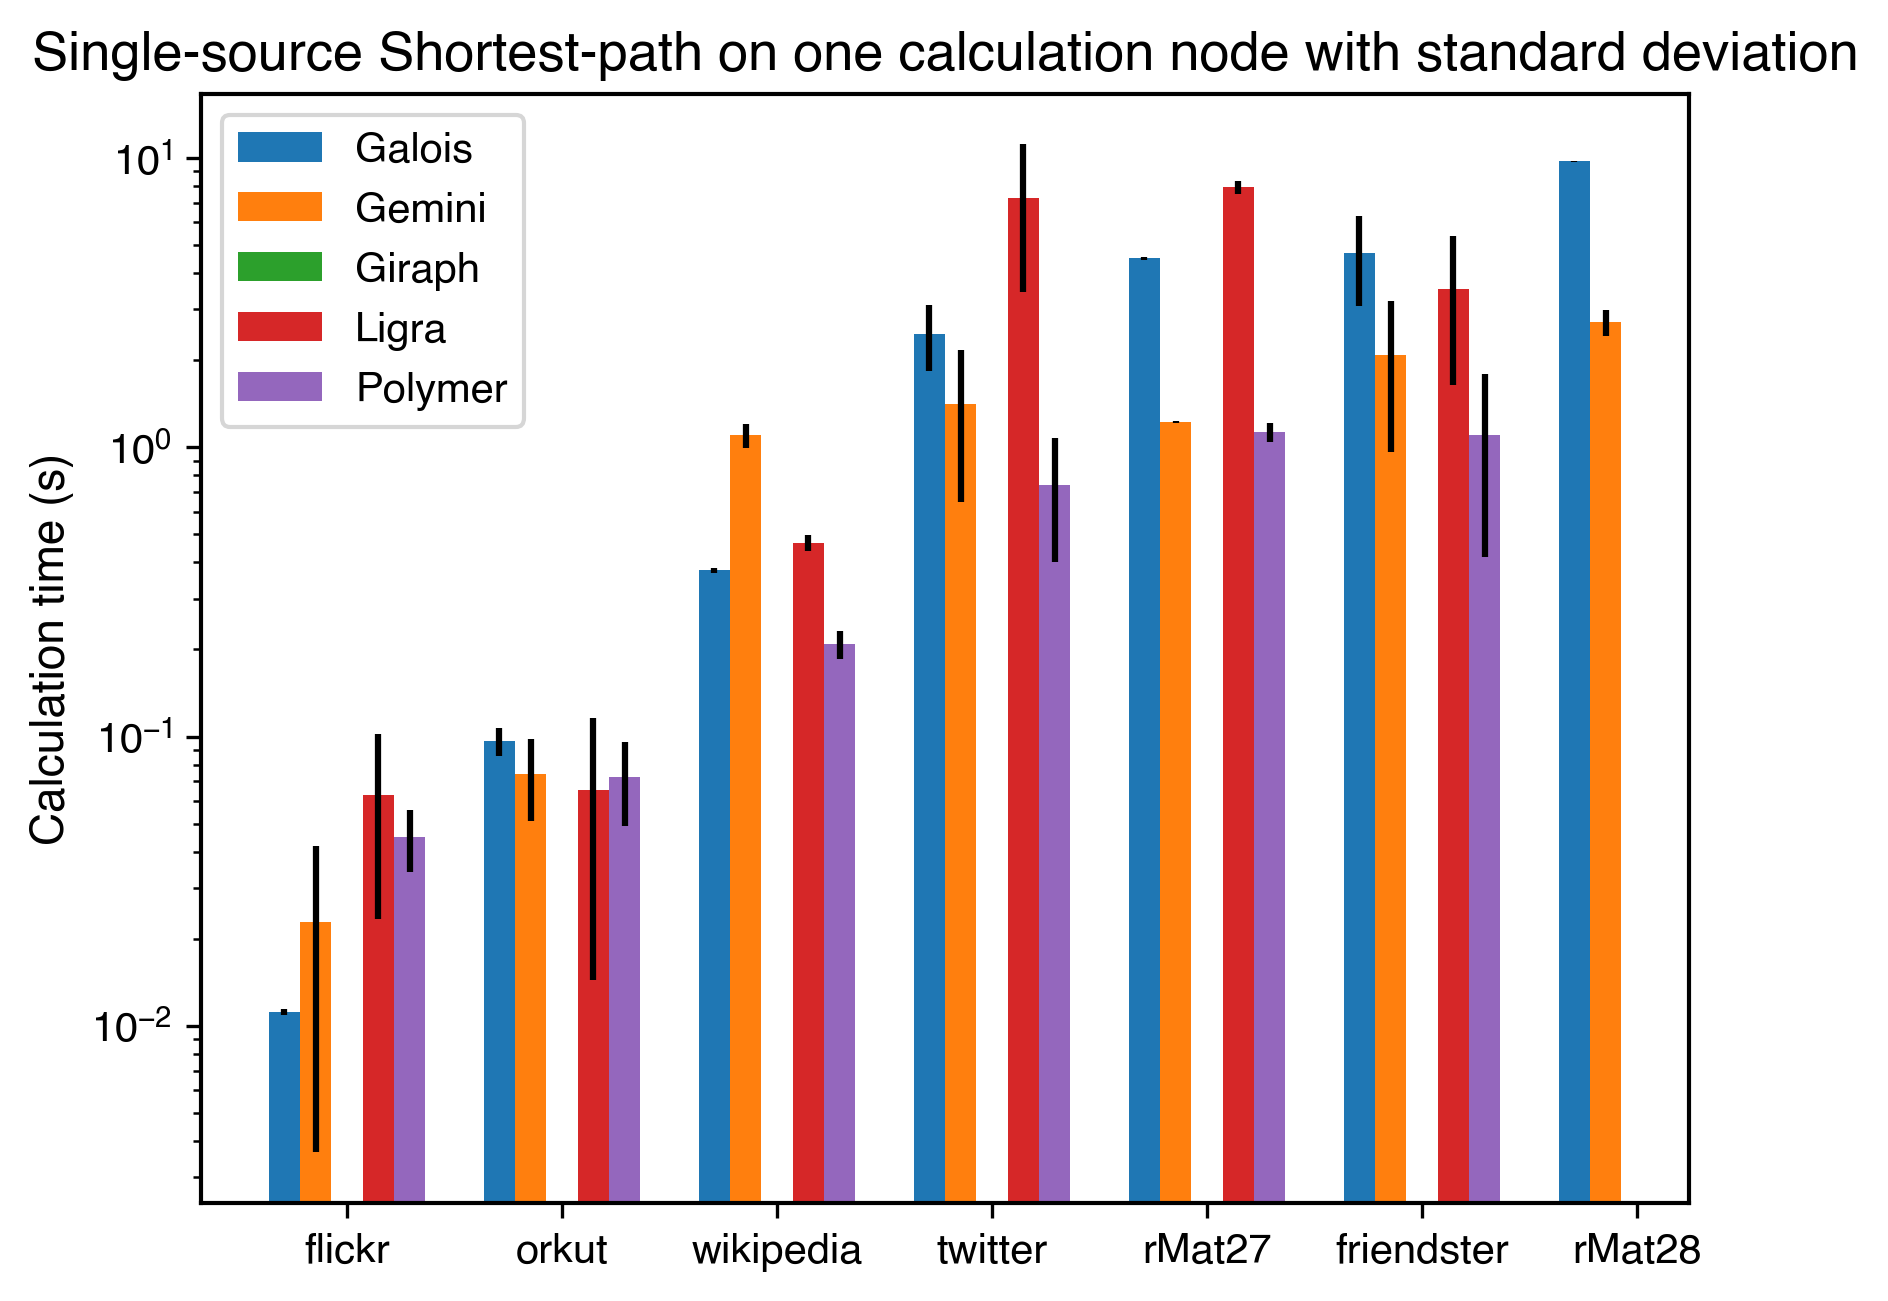
\includegraphics[width=\linewidth]{../../plots/singleNodeSSSP_calcTime.png}
		\caption{Calculation times for SSSP on a single node}
		\label{fig:singleNodeSSSP_calc}
	\end{subfigure}
	\hfil
	\begin{subfigure}{0.3\textwidth}
		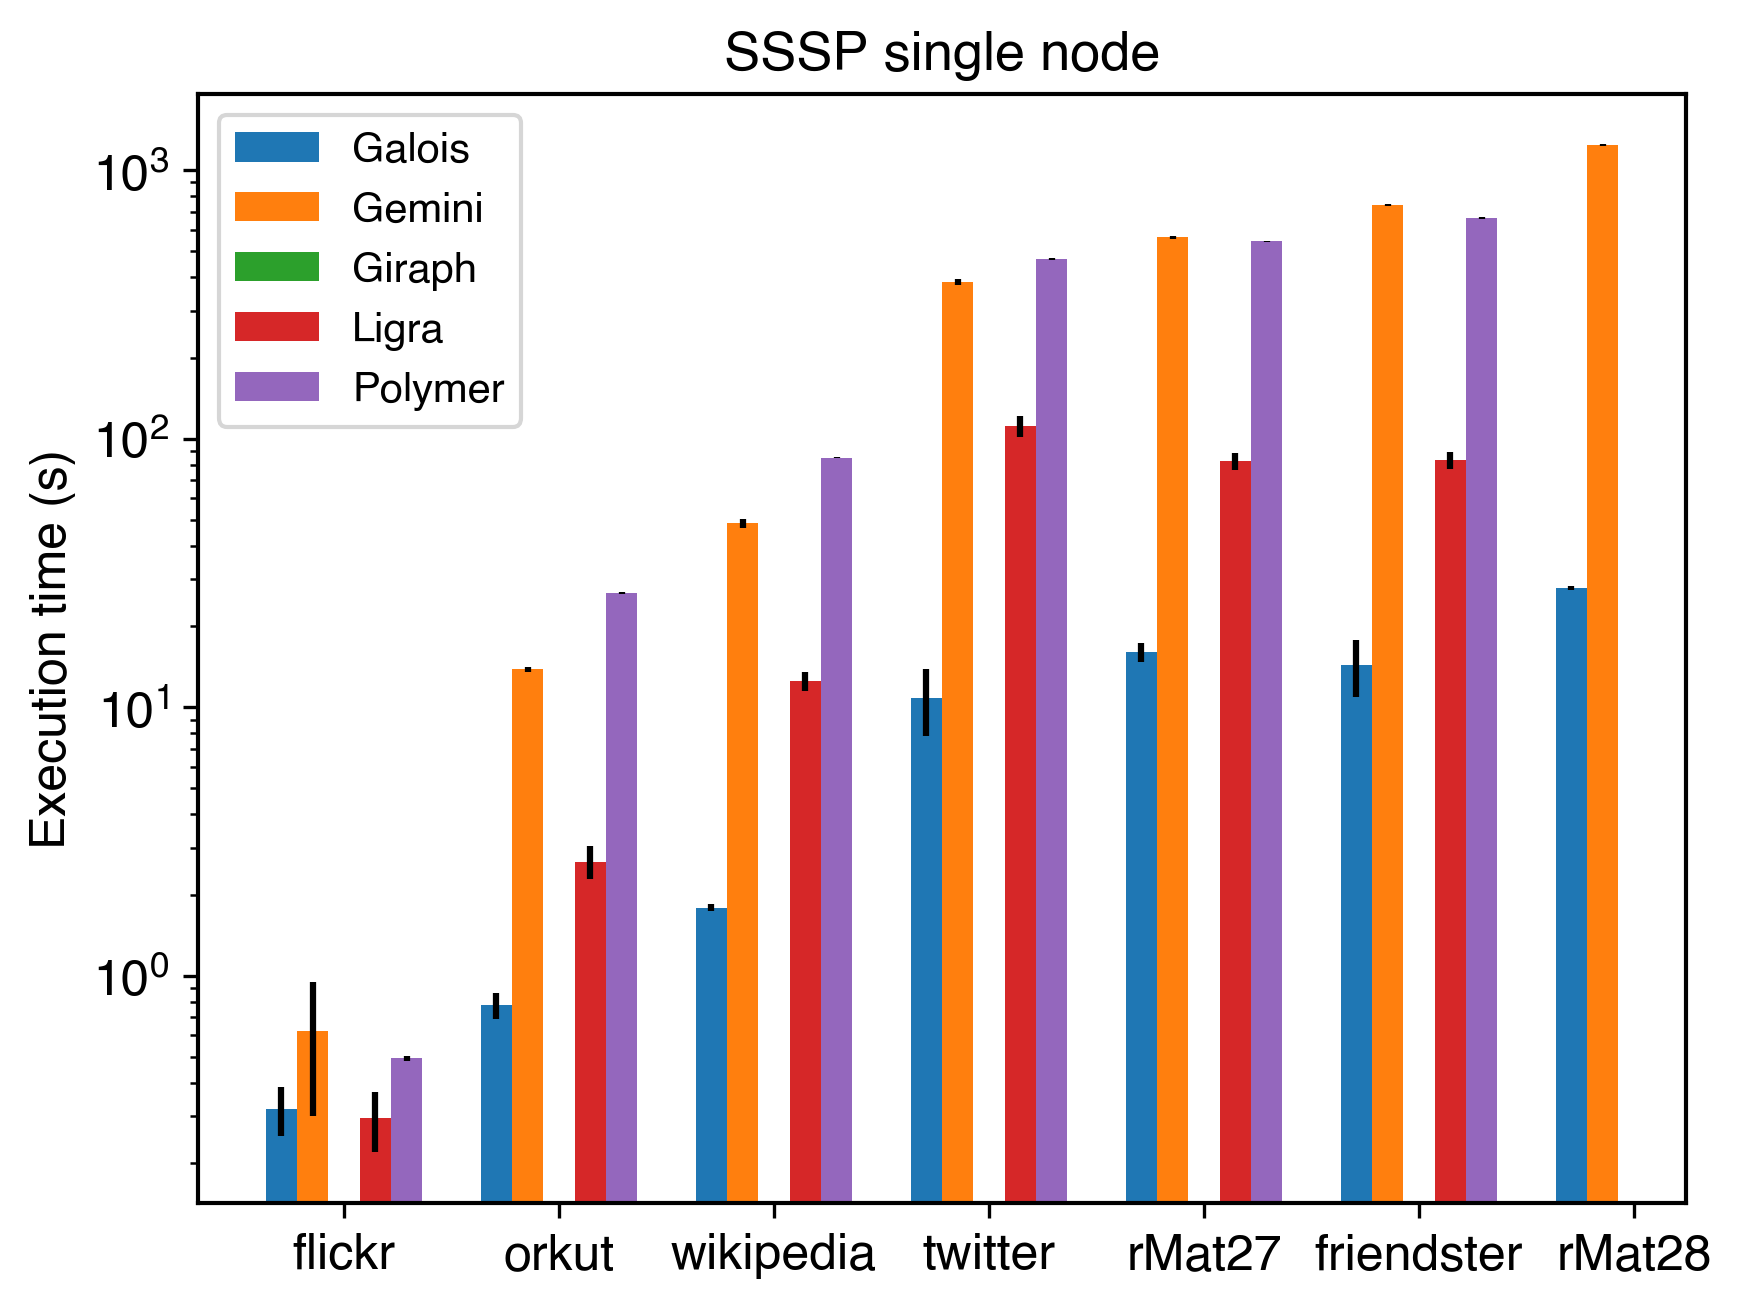
\includegraphics[width=\linewidth]{../../plots/singleNodeSSSP_execTime.png}
		\caption{Execution times for SSSP on a single node}
		\label{fig:singleNodeSSSP_exec}
	\end{subfigure}
	\hfil
	\begin{subfigure}{0.3\textwidth}
		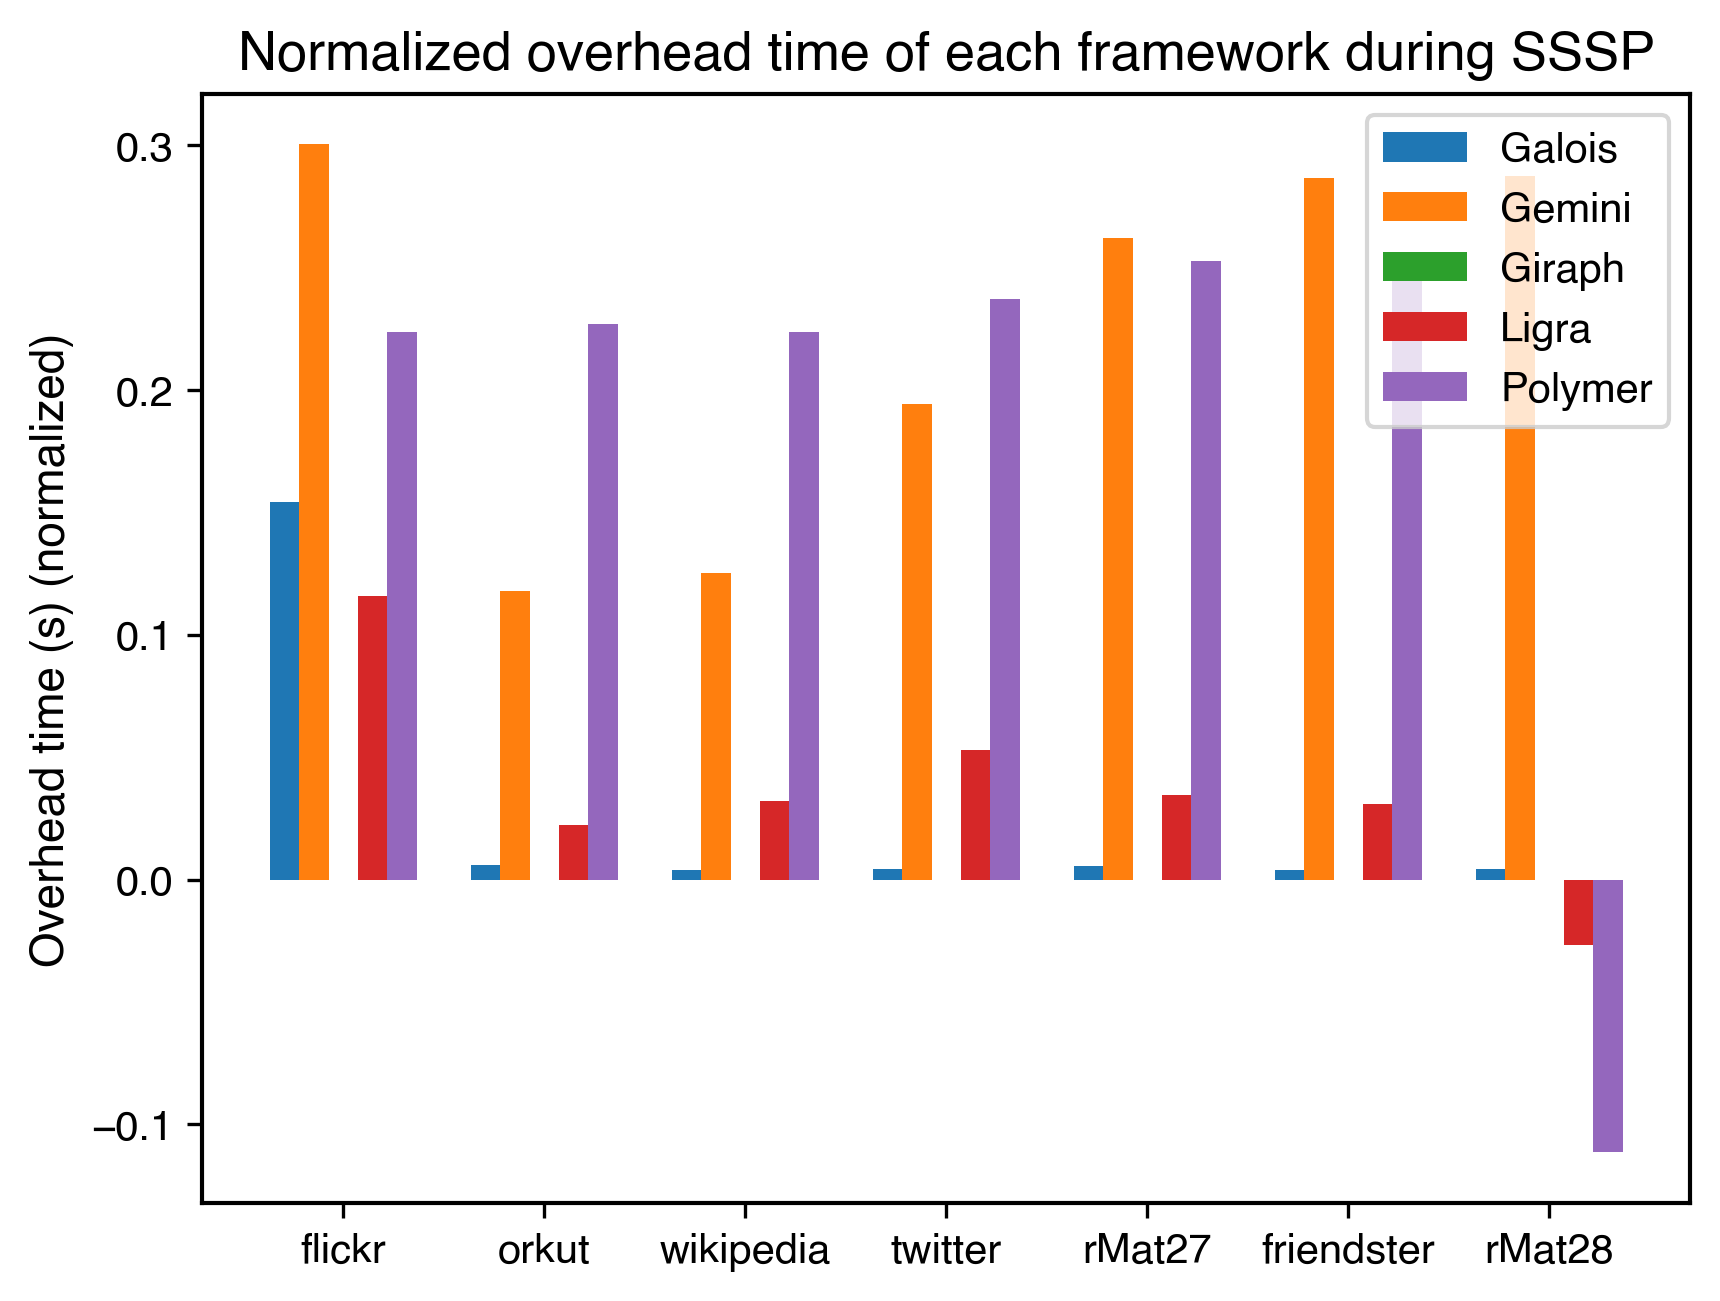
\includegraphics[width=\linewidth]{../../plots/singleNodeSSSP_overheadTimeNormalized.png}
		\caption{Overhead time normalized by the graph size in million edges}
		\label{fig:singleNodeSSSP_overheadNormalized}
	\end{subfigure}
	\caption{Average times on a single computation node, black bars represent one standard deviation in our testing.
	The runs on rMat28 for Ligra and Polymer failed and the frameworks were unable to complete the task.}
	\label{fig:singleNodeSSSP}
\end{figure}








\subsubsection{Distributed}

\begin{figure}
	\centering
	\begin{subfigure}{\columnwidth}
		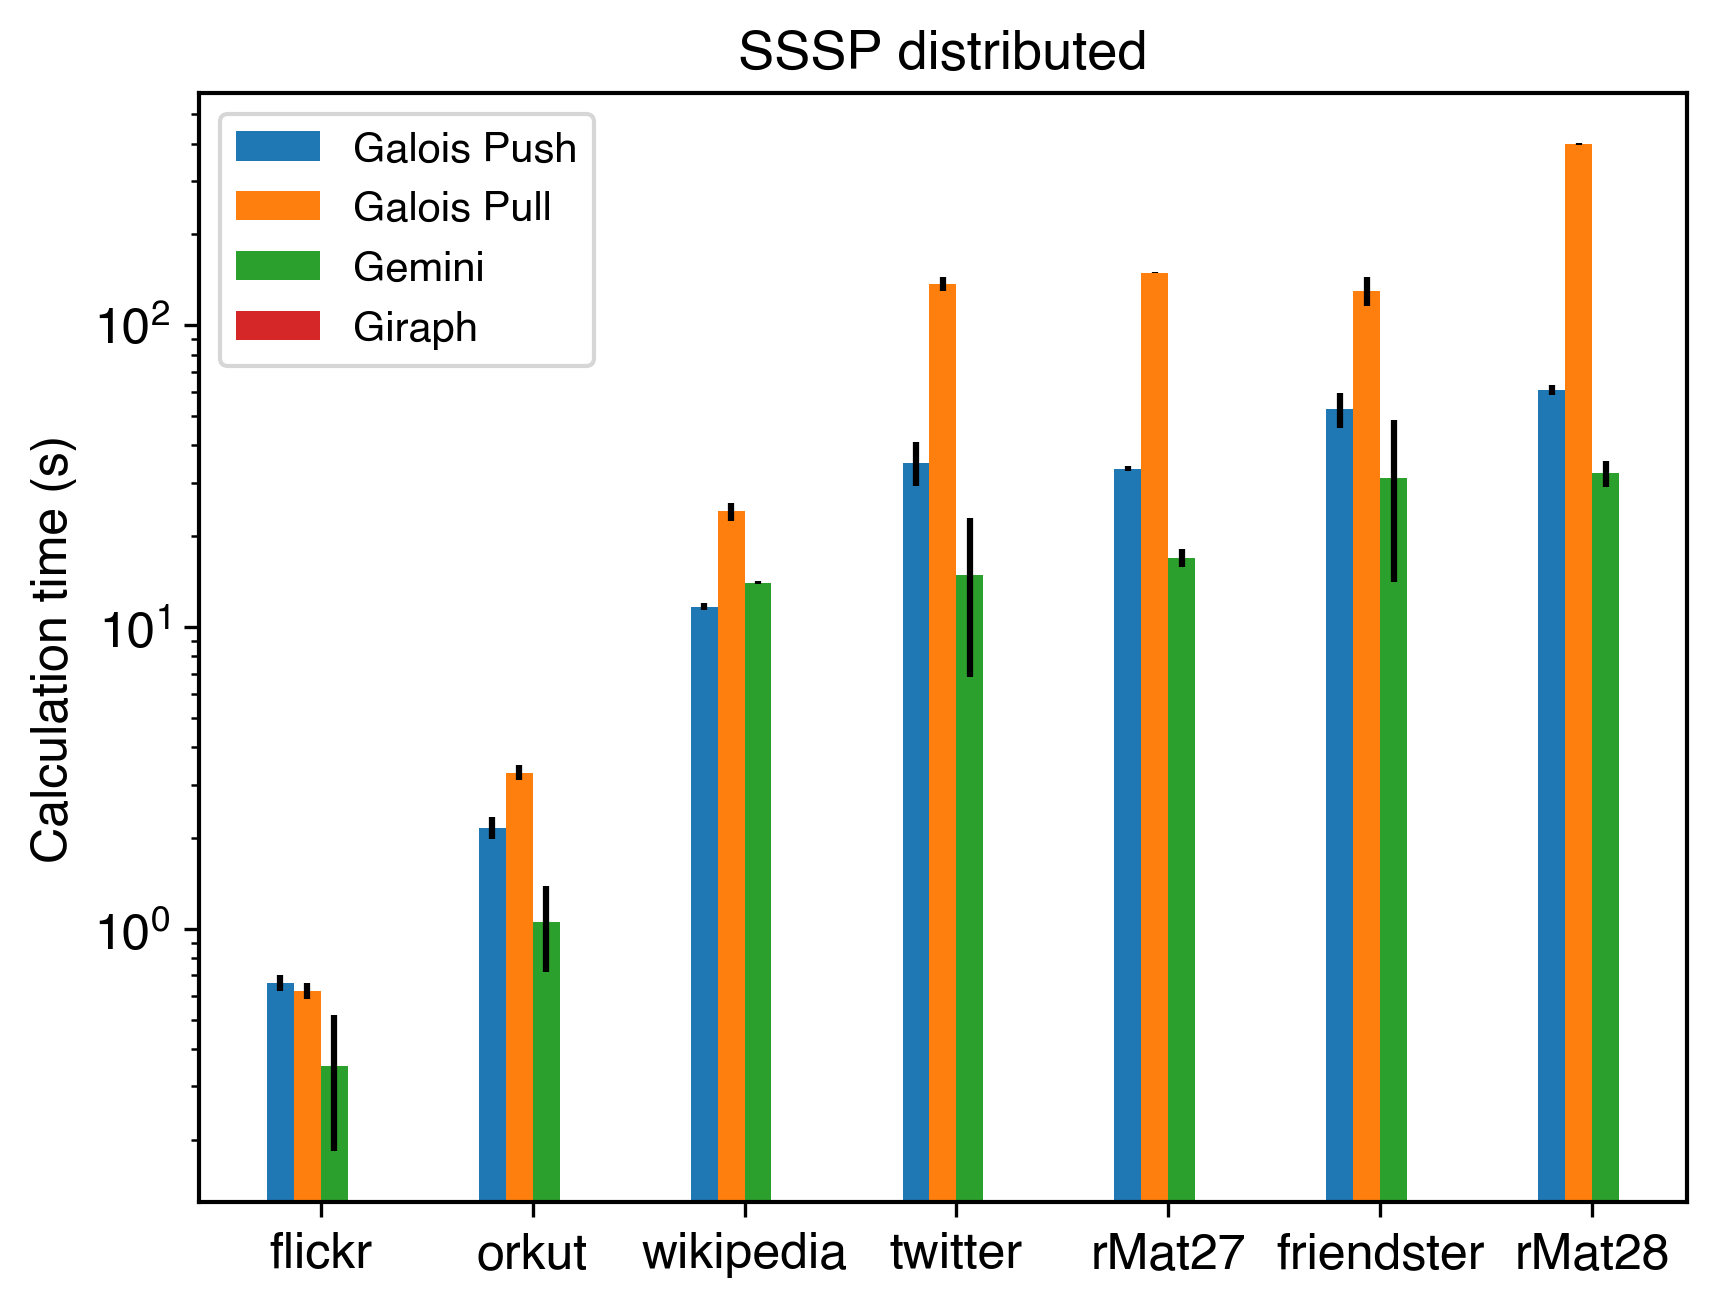
\includegraphics[width=\linewidth]{../../plots/distributedSSSP_calcTime.png}
		\caption{Calculation times for distributed SSSP}
		\label{fig:distributedSSSP_calc}
	\end{subfigure}
	\begin{subfigure}{\columnwidth}
		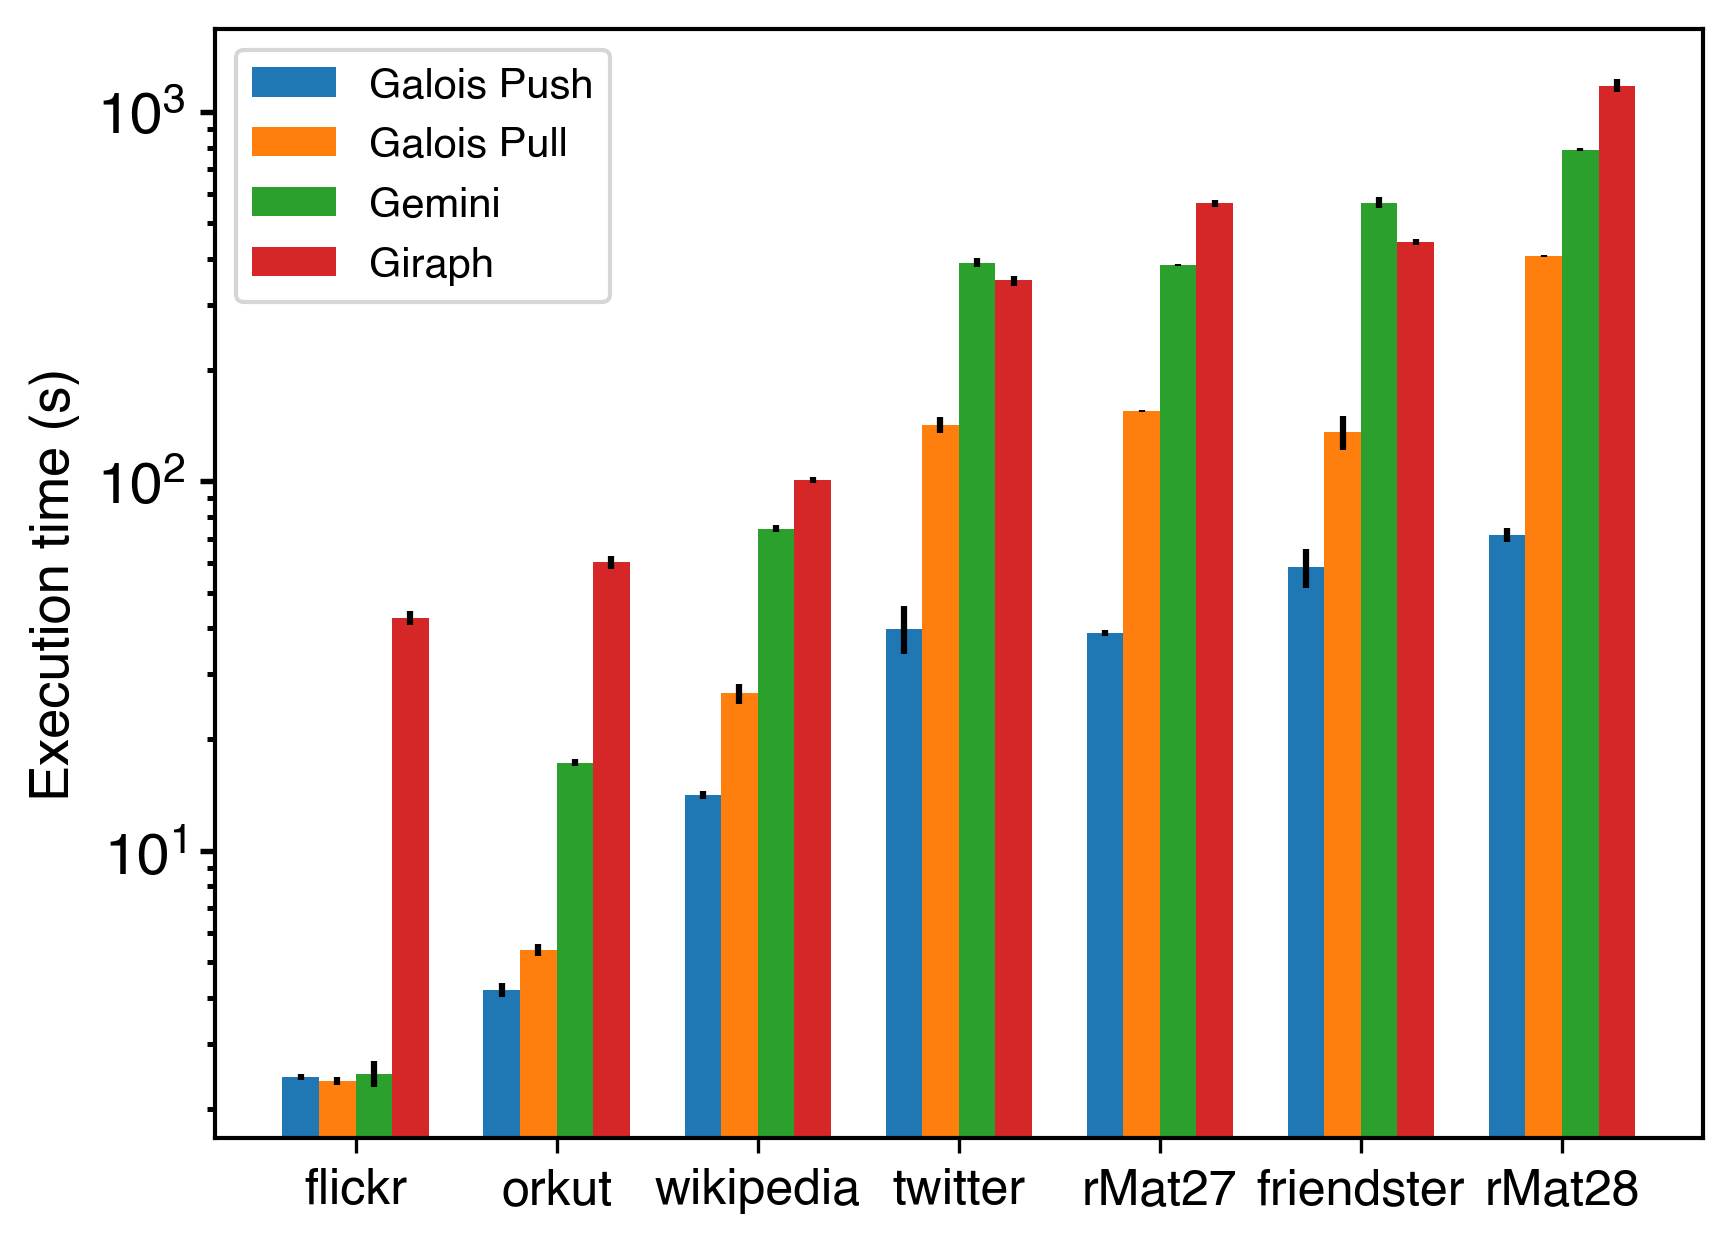
\includegraphics[width=\linewidth]{../../plots/distributedSSSP_execTime.png}
		\caption{Execution times for distributed SSSP}
		\label{fig:distributedSSSP_exec}
	\end{subfigure}
	\caption{Average times on the distributed cluster, black bars represent one standard deviation in our testing.}
	\label{fig:distributedSSSP}
\end{figure}

\begin{figure}
	\centering
	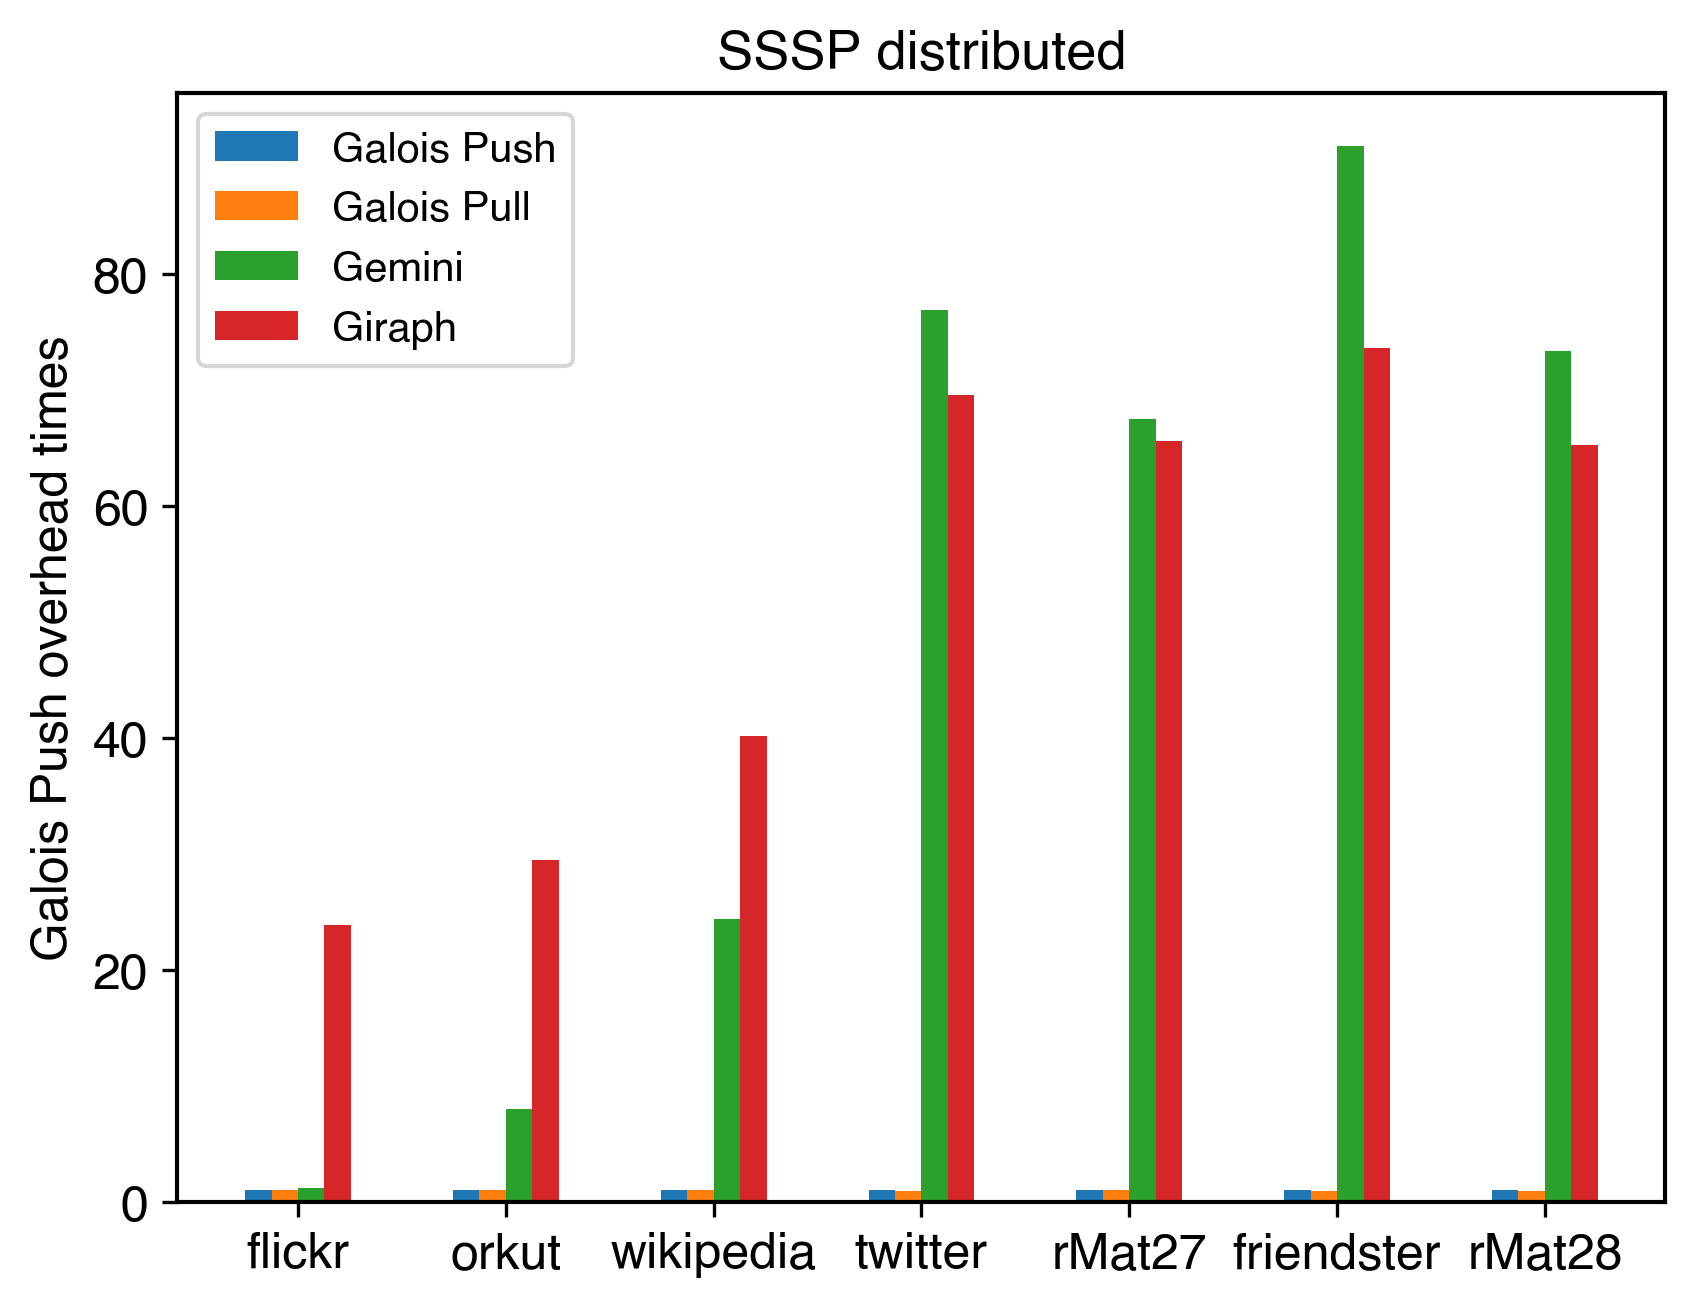
\includegraphics[width=\linewidth]{../../plots/distributedSSSP_overheadTimeNormalizedToGalois.png}
	\caption{Distributed Single-Source Shortest-Paths overhead times of each framework normalized by the overhead time of Galois Push}
	\label{fig:distributedSSSP_overhead}
\end{figure}

Moving on to the distributed cluster, \autoref{fig:distributedSSSP} shows the benchmark results as calculation and execution times. 

Comparing the two Galois implementations, we find the calculation and execution times to be similar on smaller graphs and Push being the superior implementation for SSSP on larger data sets. Galois Pull being anywhere from just as fast to 3.5$\times$ slower on real-world data sets compared to the Push variant. The synthetic graphs are more extreme, execution times are close to 4$\times$ (rMat27) and 5$\times$ (rMat28) longer.

Both Galois implementations have significantly smaller execution times compared to Gemini or Giraph on all graphs, see \autoref{tbl:ssspexec}.
You can see Gemini being worse by at least a factor of 4 compared to Galois Push on all graphs except flickr.
Giraph's execution times in comparison to this are even worse, taking at least 7$\times$ longer than Galois Push on all graphs.

Evidently, Galois Push is the fastest algorithm in our lineup on 6 out of 7 graphs. With the exception being flickr, where Galois Push takes negligibly longer than the Pull counterpart. 



\begin{table}
\renewcommand{\arraystretch}{1.3}
\centering
\caption{Distributed SSSP Execution Times Relative to Galois Push}
\begin{tabular}{crrrr}
\hline
\bf{Data Set}&Galois Push&Galois Pull&Gemini&Giraph\\\hline
flickr&1.0&0.97&1.02&17.46\\
orkut&1.0&1.28&4.12&14.38\\
wikipedia&1.0&1.88&5.26&7.11\\
twitter&1.0&3.56&9.79&8.76\\
rMat27&1.0&3.98&9.91&14.52\\
friendster&1.0&2.32&9.72&7.59\\
rMat28&1.0&5.70&11.07&16.5\\\hline
\end{tabular}
\label{tbl:ssspexec}
\end{table}



When taking a closer look at Giraph, it seems to not cope well with synthetic data sets. Analyzing the computation times in \autoref{fig:distributedSSSP_calc}, we see that it is the fastest framework on our real-world graphs. And that with a considerable margin of other frameworks always taking at least 50\% longer (lower bound here is Gemini on flickr) up to Galois Pull needing 18$\times$ more time on wikipedia.  
On both synthetic graphs however, Giraph is actually the slowest to compute. Giraph requires 12$\times$ or even 15$\times$ the computation time of Gemini on rMat27 or rMat28 respectively.

While Giraph's computation times are very competitive, when comparing the execution times in \autoref{fig:distributedSSSP_exec} we see that Giraph is actually the slowest framework on 5 out of 7 graphs. For the other two, namely twitter and friendster, Giraph is second slowest with only Gemini taking longer to complete.

Giraph and Gemini's very long execution times are only due to their overhead being many orders of magnitude larger than Galois overhead (\autoref{fig:distributedSSSP_overhead}).
Overhead for Gemini is greater than that of Galois on every graph. From just a 20\% increase on flickr up to friendster, where the overhead is 90$\times$ that of Galois Push.
For Giraph the overhead times are not as extreme but still generally worse. Even on flickr, Giraph's overhead time is already 23$\times$ that of Galois. On friendster, where Gemini was worst, Giraph \emph{only} requires 73$\times$ the overhead time of Galois.



\subsubsection{Single-Node vs. Distributed}
TODO
\begin{itemize}
	\item GaloisPush vs Galois CPU // Galois Pull verliert bei Dist.
	\item Giraph vs. Giraph
	\item Gemini vs Gemini
\end{itemize}




%!TEX root=../../main.tex

\subsection{Breadth-first search}
\subsubsection{Single-Node}
\todo{Hier fehlt noch Giraph, daher noch keine vollständige Auswertung.}


In these figures, Galois with 96 threads is shown. Again, we show the impact of Galois' thread count in \autoref{sec:galois_speedup}.
\begin{figure*}
	\begin{subfigure}{0.3\textwidth}
		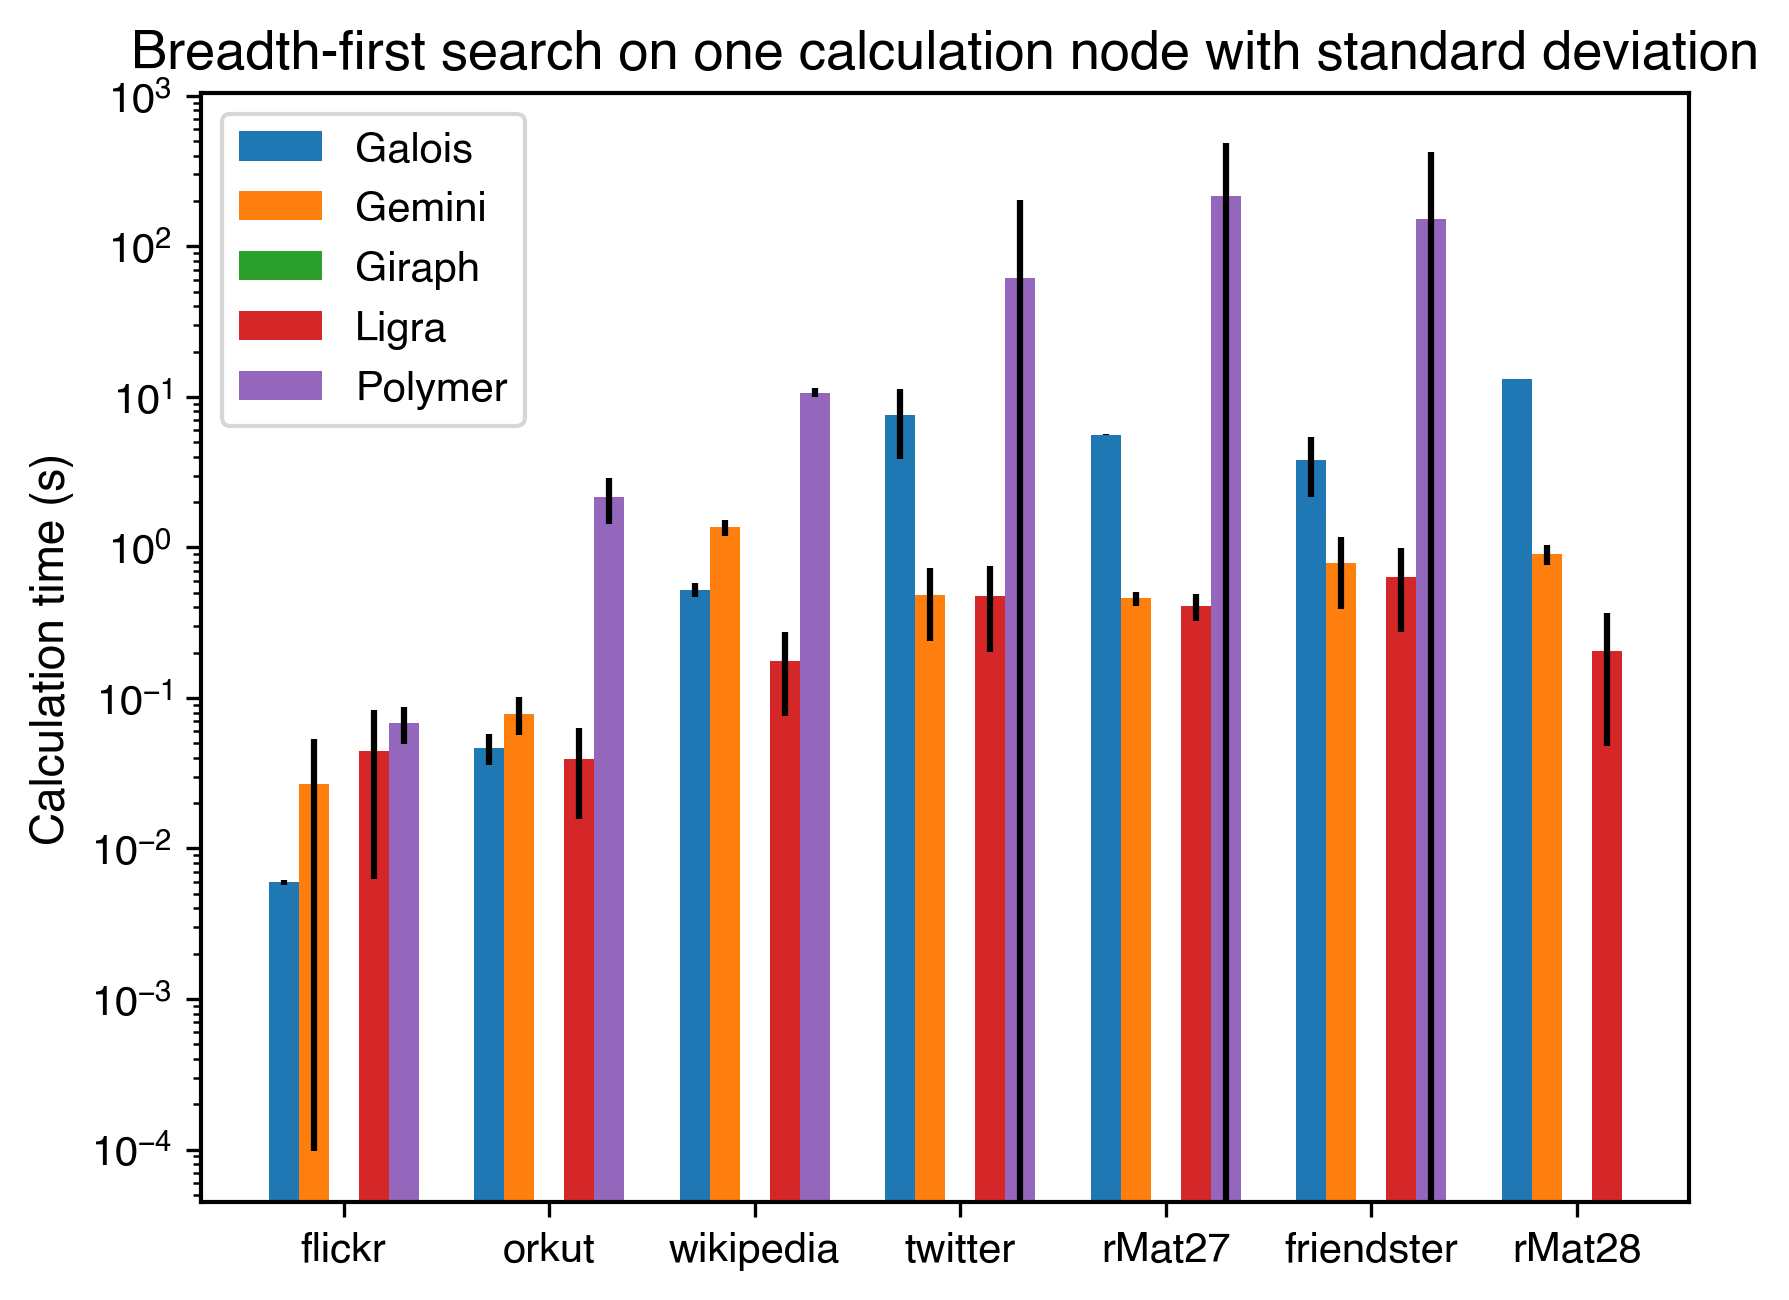
\includegraphics[width=\linewidth]{../../plots/singleNodeBFS_calcTime.png}
		\caption{Calculation times for BFS on a single node}
		\label{fig:singleNodeBFS_calc}
	\end{subfigure}
	\hfil
	\begin{subfigure}{0.3\textwidth}
		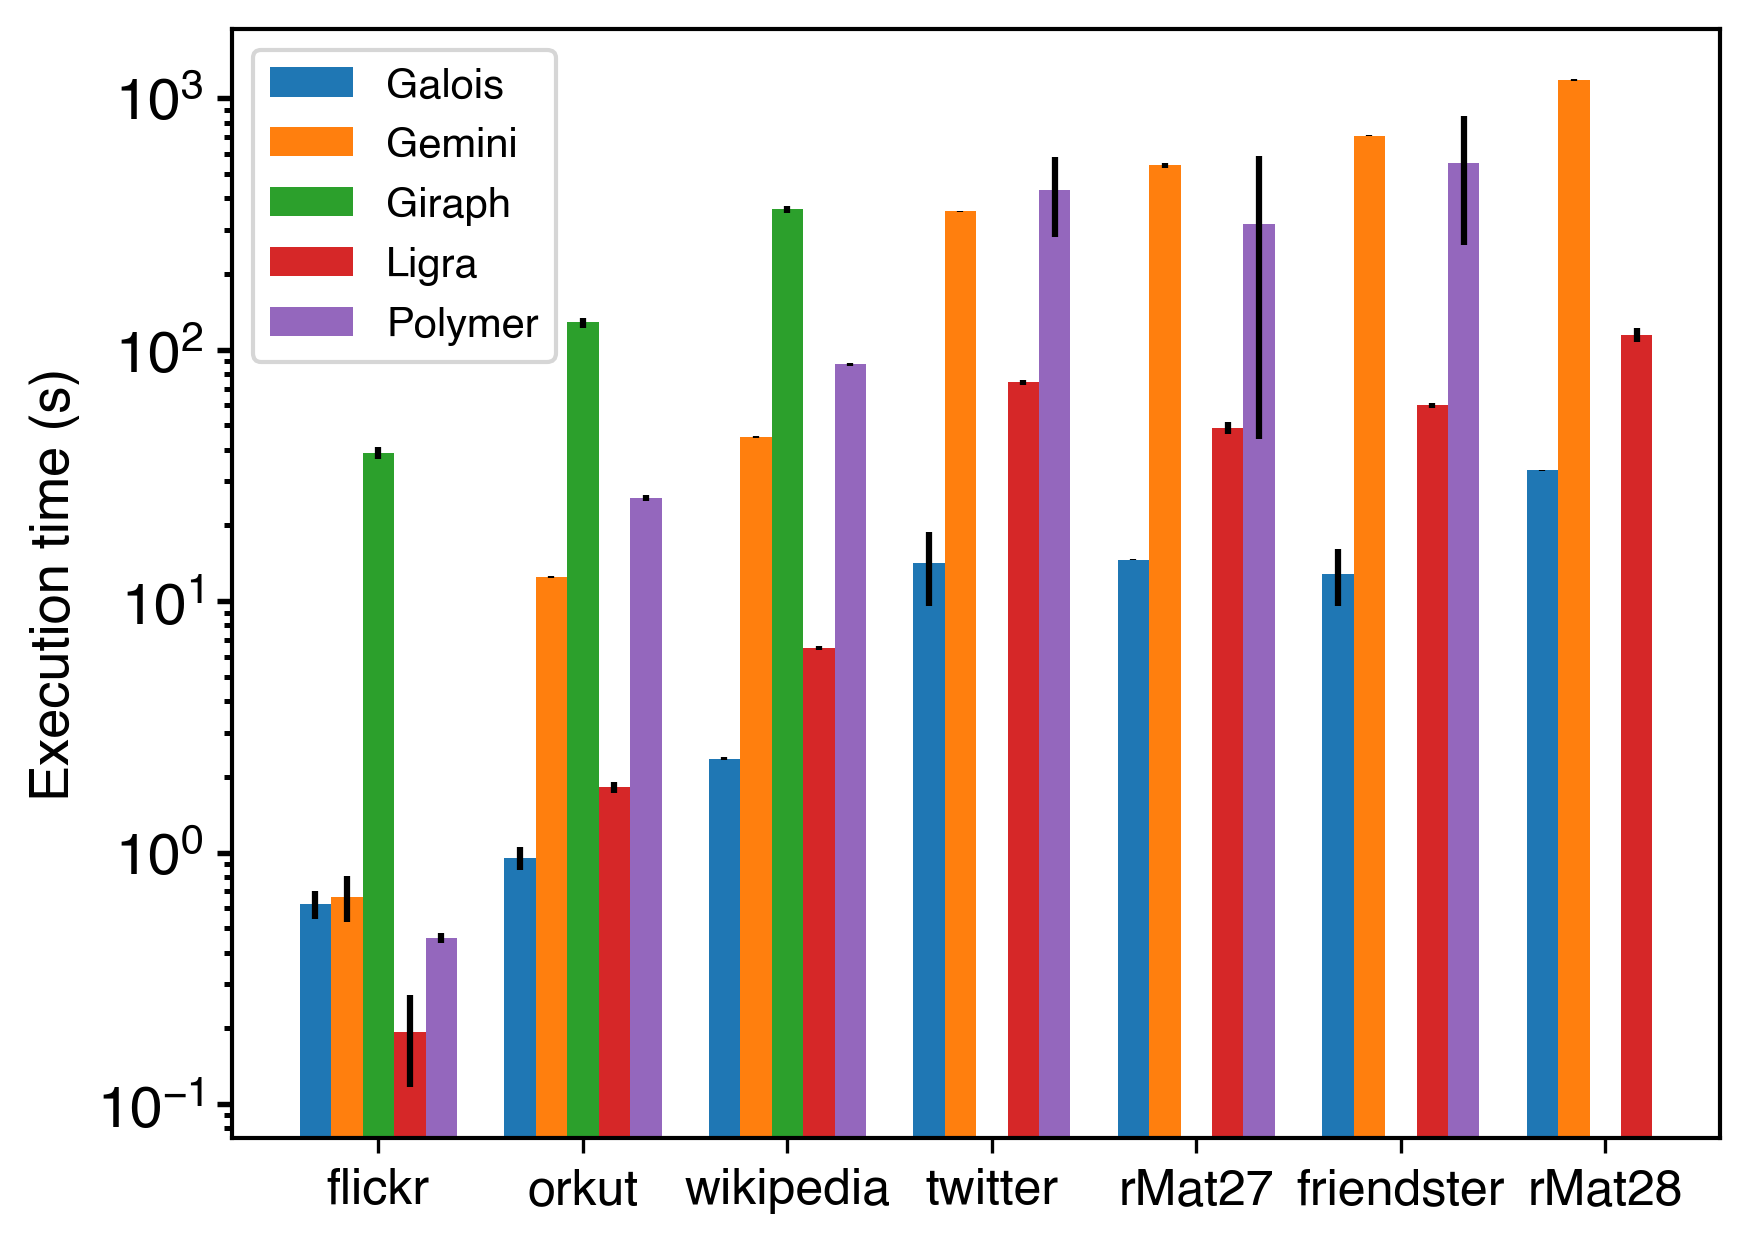
\includegraphics[width=\linewidth]{../../plots/singleNodeBFS_execTime.png}
		\caption{Execution times for BFS on a single node}
		\label{fig:singleNodeBFS_exec}
	\end{subfigure}
	\hfil
	\begin{subfigure}{0.3\textwidth}
		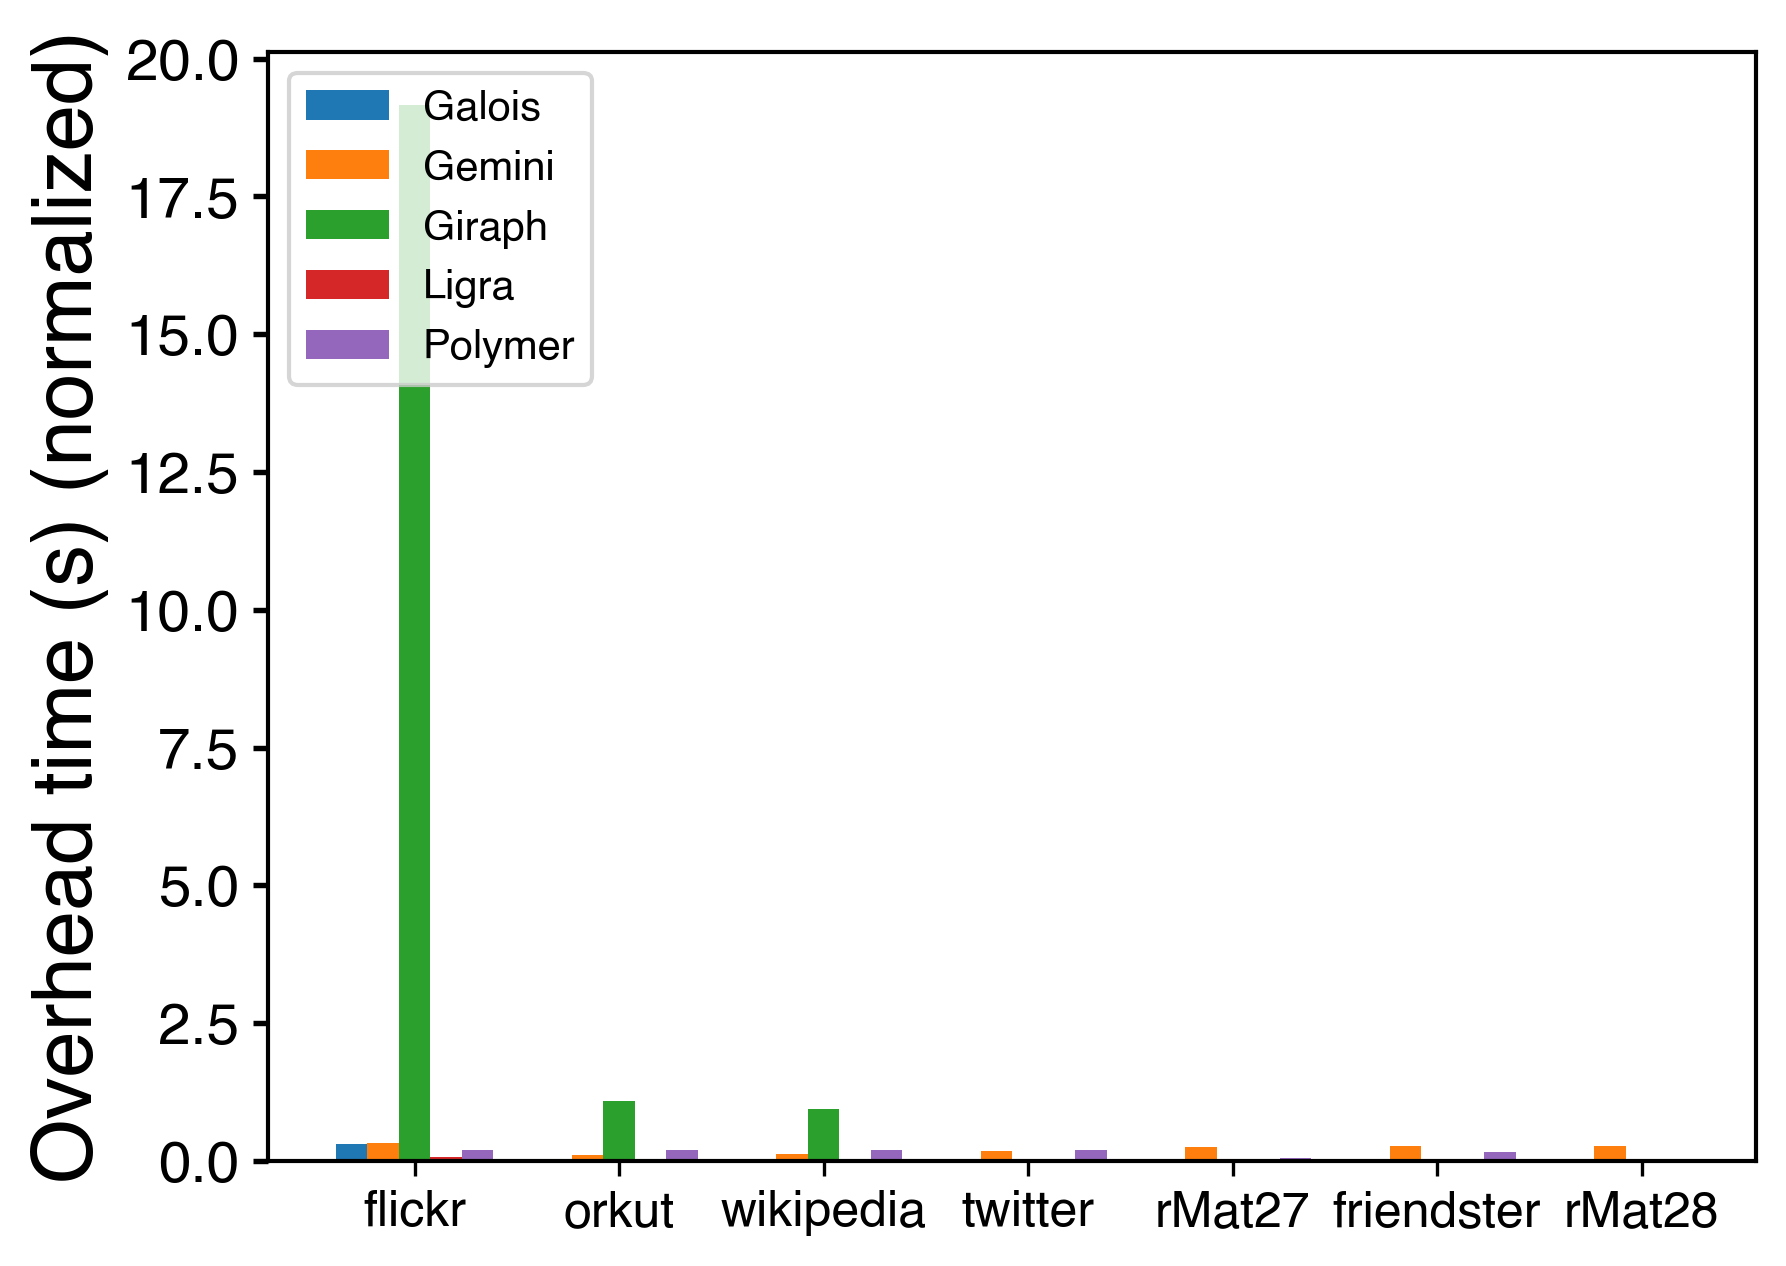
\includegraphics[width=\linewidth]{../../plots/singleNodeBFS_overheadTimeNormalized.png}
		\caption{Overhead time normalized by the graph size in million edges}
		\label{fig:singleNodeBFS_overheadNormalized}
	\end{subfigure}

	\caption{Average times on a single computation node, black bars represent one standard deviation in our testing}
\end{figure*}



\subsubsection{Distributed}
\begin{figure}
	\begin{subfigure}{\columnwidth}
		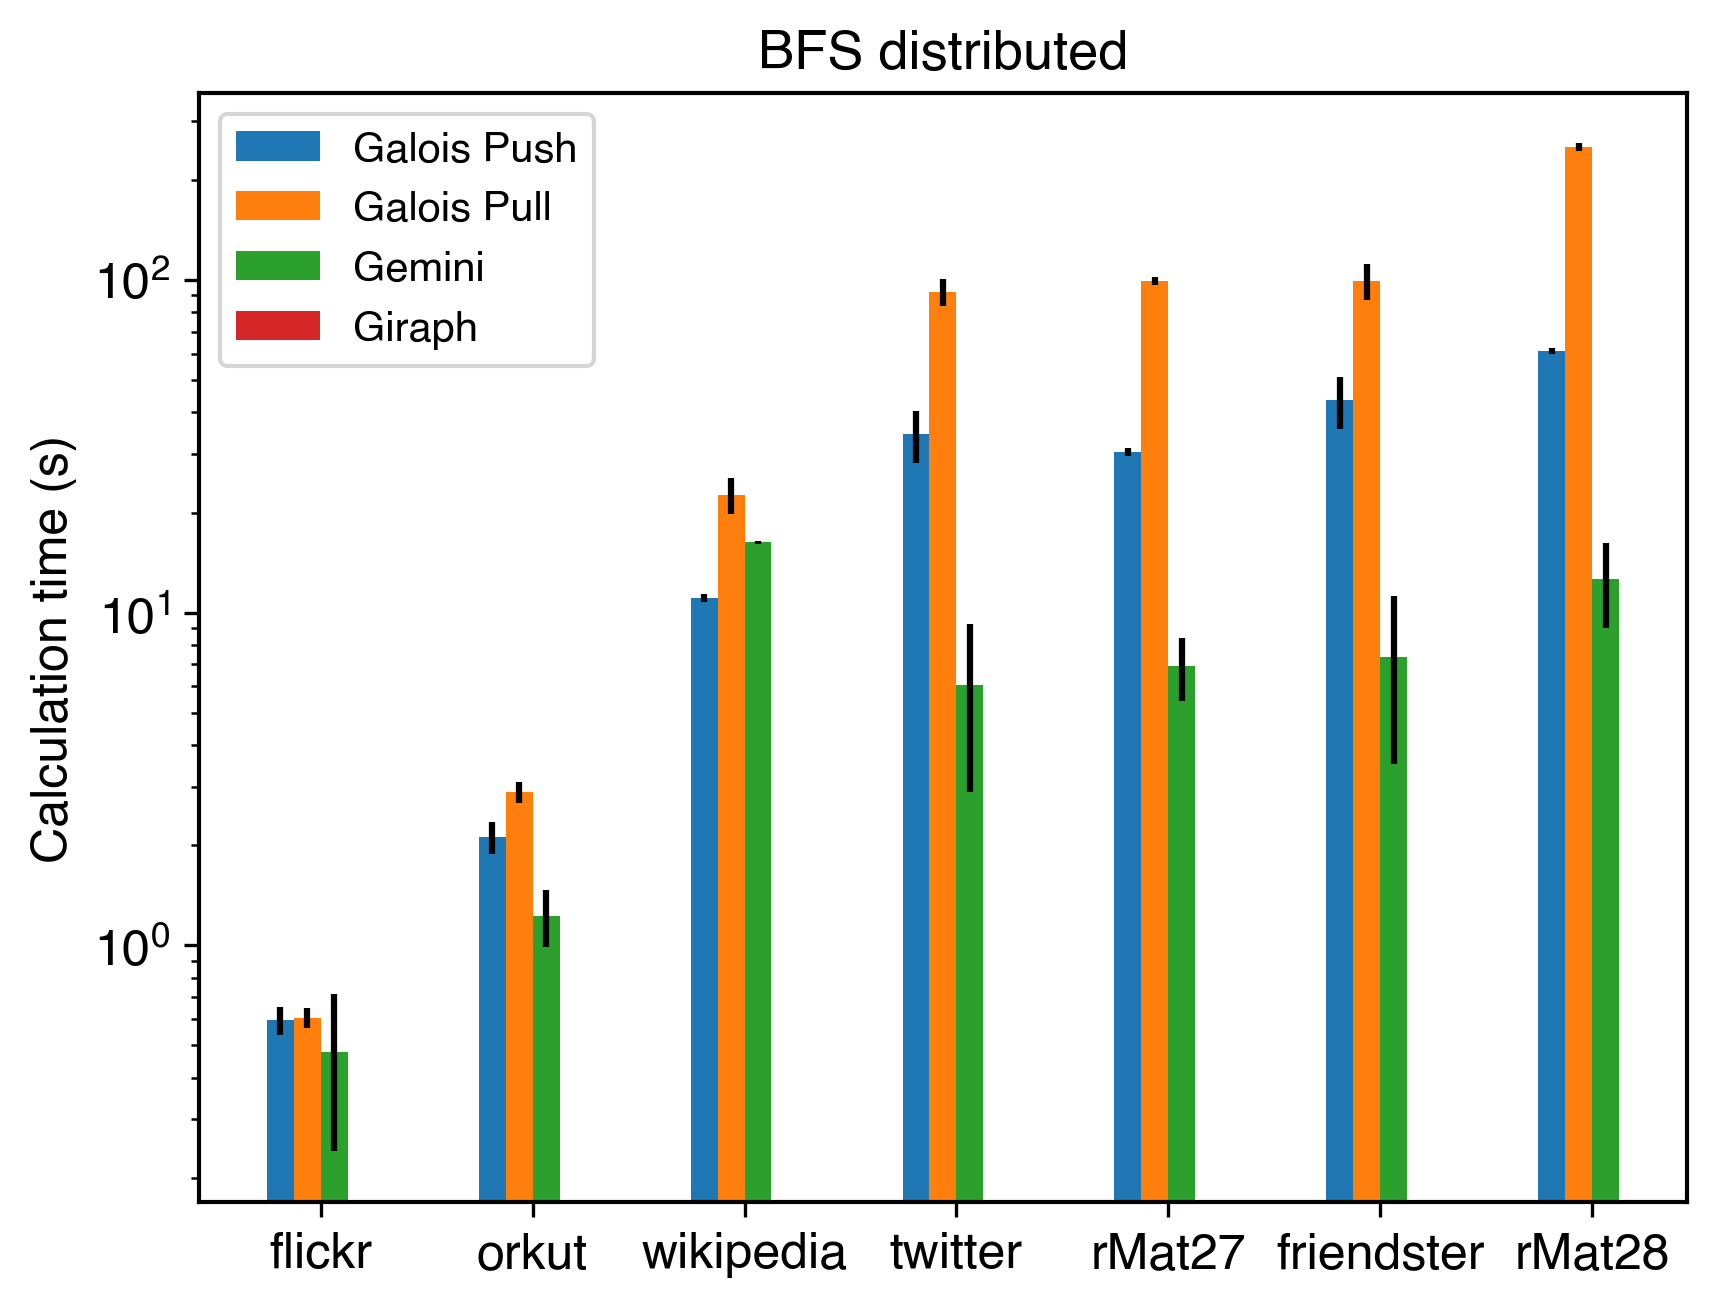
\includegraphics[width=\linewidth]{../../plots/distributedBFS_calcTime.png}
		\caption{Calculation times for distributed BFS}
		\label{fig:distributedBFS_calc}
	\end{subfigure}
	% \hfil
	\begin{subfigure}{\columnwidth}
		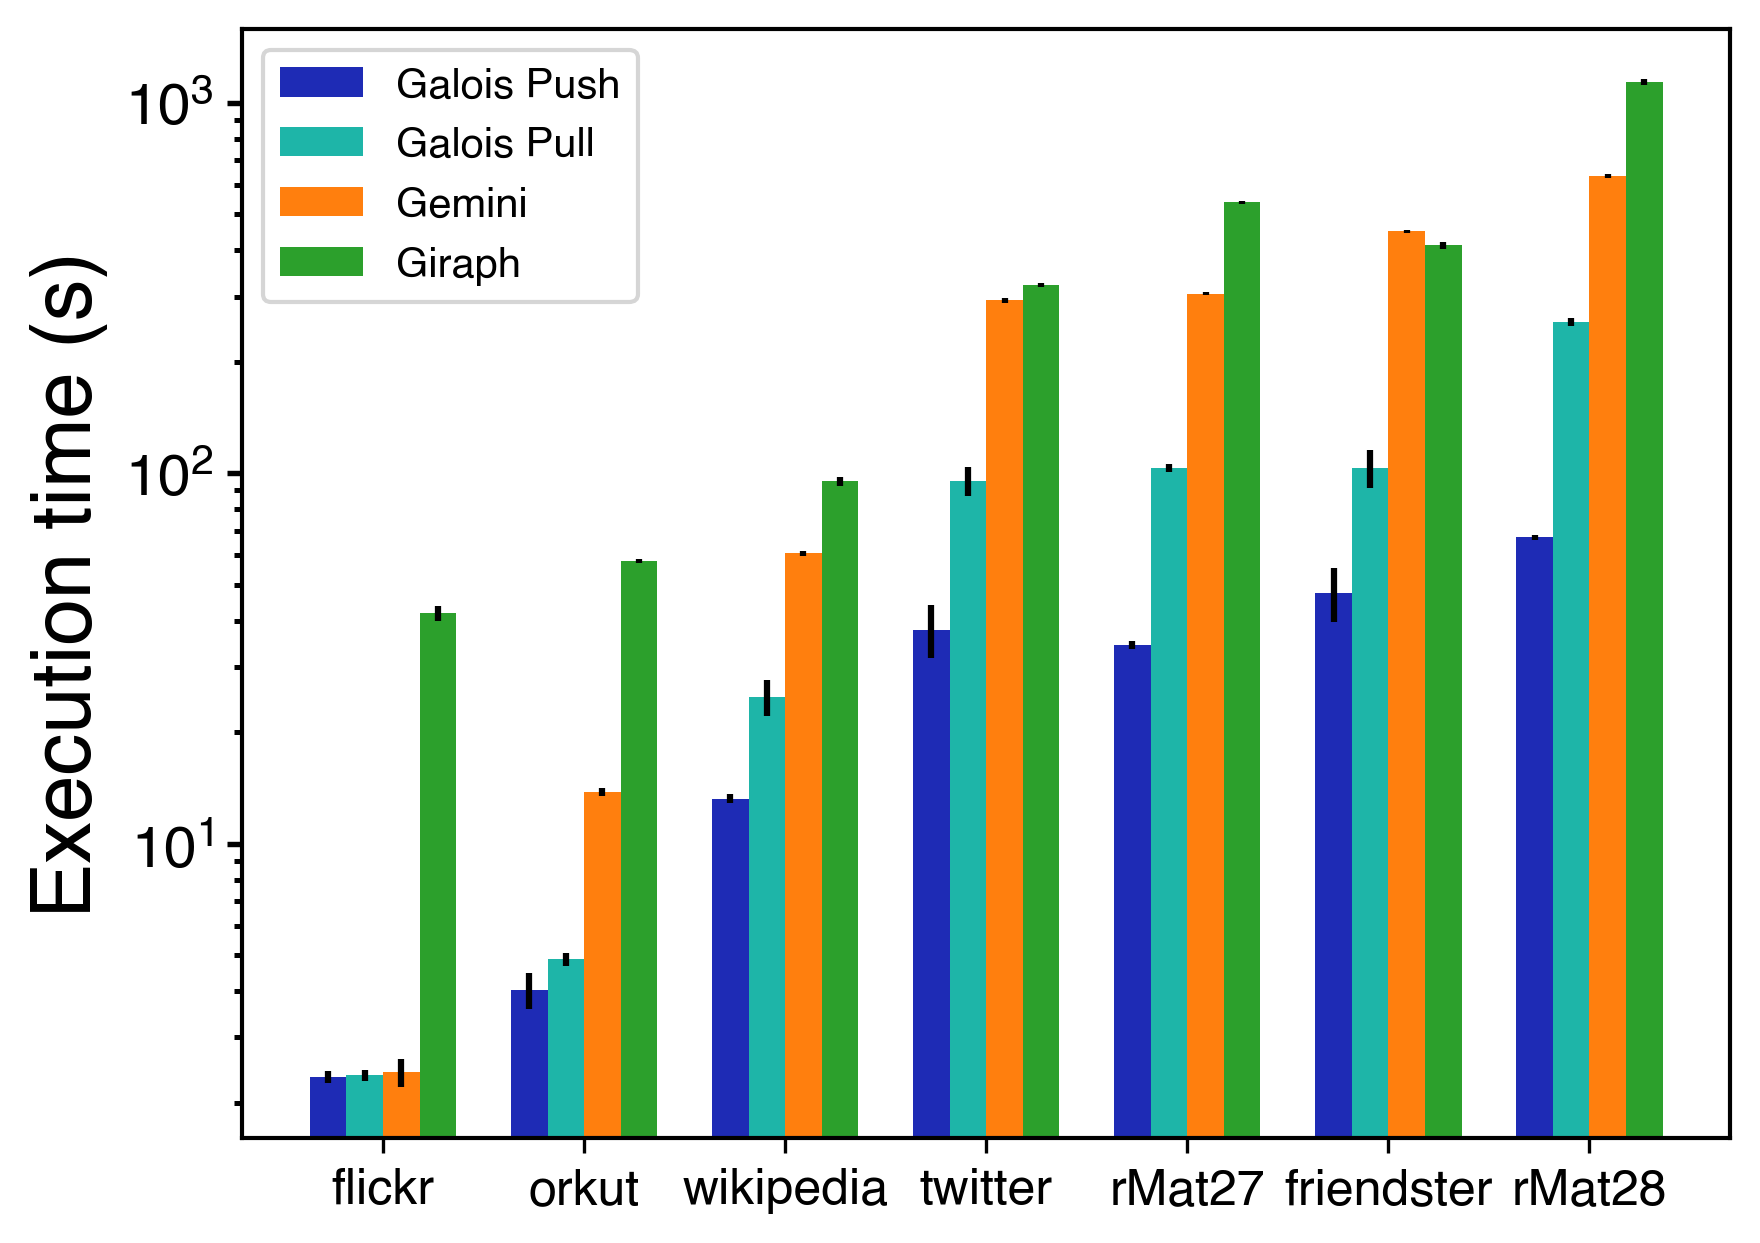
\includegraphics[width=\linewidth]{../../plots/distributedBFS_execTime.png}
		\caption{Execution times for distributed BFS}
		\label{fig:distributedBFS_exec}
	\end{subfigure}
	% \hfil
	% \begin{subfigure}{0.3\textwidth}
	% 	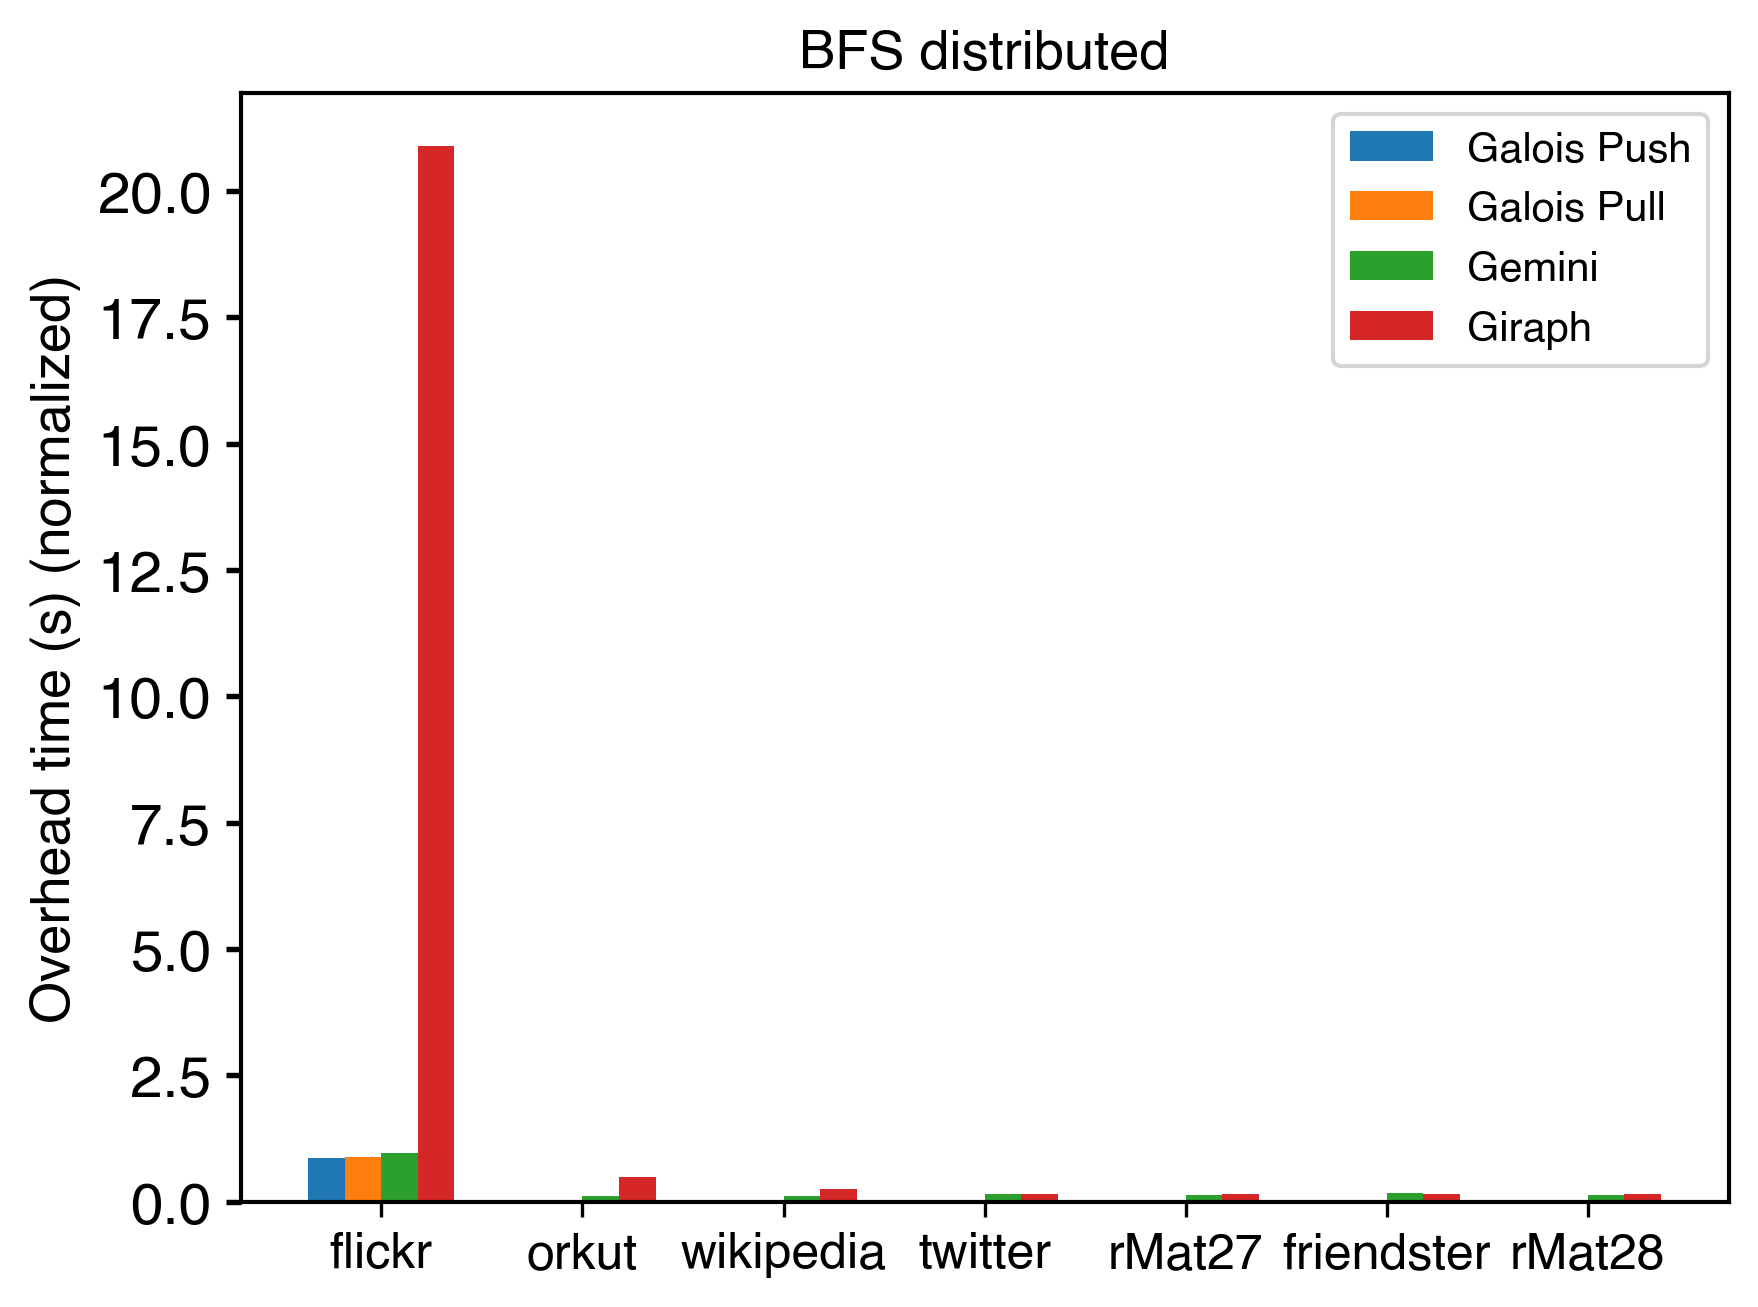
\includegraphics[width=\linewidth]{../../plots/distributedBFS_overheadTimeNormalized.png}
	% 	\caption{Overhead time normalized by the graph size in million edges}
	% 	\label{fig:distributedBFS_overheadNormalized}
	% \end{subfigure}
	\caption{Average times on the distributed cluster, black bars represent one standard deviation in our testing}
	\label{fig:distributedBFS}
\end{figure}
For both the calculation and the execution times, Breadth-First Search shows similar behaviour as the distributed SSSP test case. This is expected since both are graph traversal algorithms starting in one source vertex.
Hence, calculation complexity for each vertex and communication overhead is similar.
All measurements can be seen in \autoref{fig:distributedBFS}.

First, the calculation times in \autoref{fig:distributedBFS_calc}. It shows Giraph having the shortest calculation times on the real-world graphs, while Giraph's calculatin times on both rMat27 and rMat28 are the worst of all frameworks.

Comparing the execution times in \autoref{fig:distributedBFS_exec} results in the same findings as with SSSP.
While Gemini can compete with Galois on the small flickr graph, moving to larger data sets shows the worse performance of Gemini compared to Galois.

Much like when running SSSP, Giraph is slowest on all but one graph. Only on friendster is Gemini marginally slower, which was also the case for SSSP.

Both Galois implementations are again similar to the behaviour on SSSP.
Galois Push is generally faster than the Pull alternative while both Push and Pull versions are faster than Gemini and Giraph across all graphs.
This makes Galois Push the clear winner for distributed BFS.



%!TEX root=../../main.tex


\subsubsection{PageRank}
In this section we compare the PageRank performance of the various frameworks. As usual we begin with the single-node performance and finish by discussing the distributed variants.

\paragraph{Single-Node}
Ligra and Polymer support both regular and Delta-PageRank variants.
Ligra's regular PR implementation is faster on 4 of 7 graphs. If the regular version is slower than delta, that is only by a small difference. Explicitly, regular is slower than delta by a range of 6\% to 19\%\ on twitter, rMat27 or friendster. For the other graphs, the delta version is slower by a far greater margin of 13\% to 68\%.
Hence, we only show the results of Ligra's regular PageRank implementation in our evaluation.
For Polymer we found the delta version to be faster on all graphs except rMat28. Delta-PR is on average 15\%\ faster on the first six graphs, while only being 0.3\%\ slower on rMat28.
Thus, the following only shows Polymer's faster Delta-PR implementation.
Giraph required more than the available 250 GB of RAM on any graph larger than wikipedia, hence all of Giraph's results for the larger graphs are missing here.
\begin{figure*}
	\hfil
	\begin{subfigure}{0.32\textwidth}
		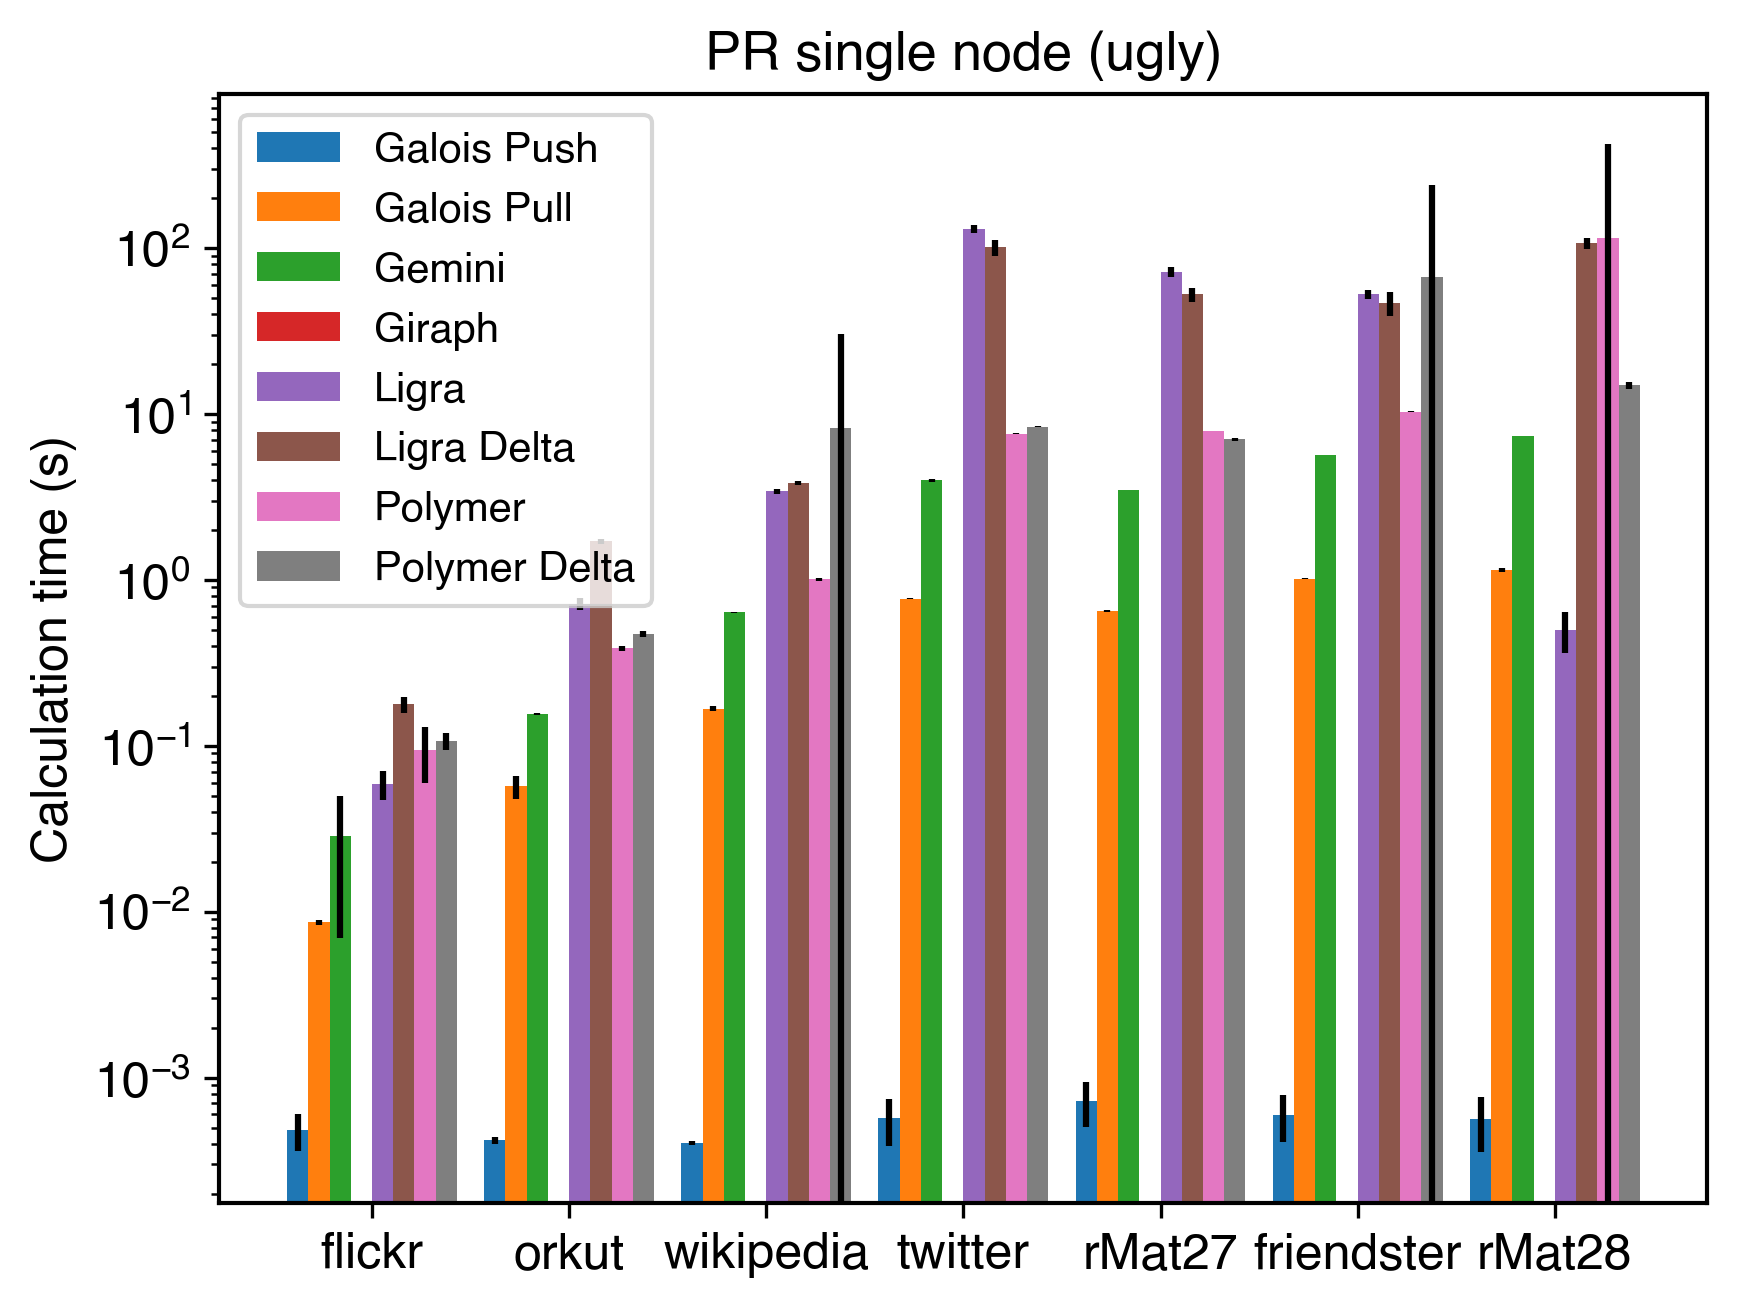
\includegraphics[width=\linewidth]{../../plots/singleNodePR_calcTime.png}
		\caption{Calculation time}
		\label{fig:singleNodePR_calc}
	\end{subfigure}
	\hfil
	\begin{subfigure}{0.32\textwidth}
		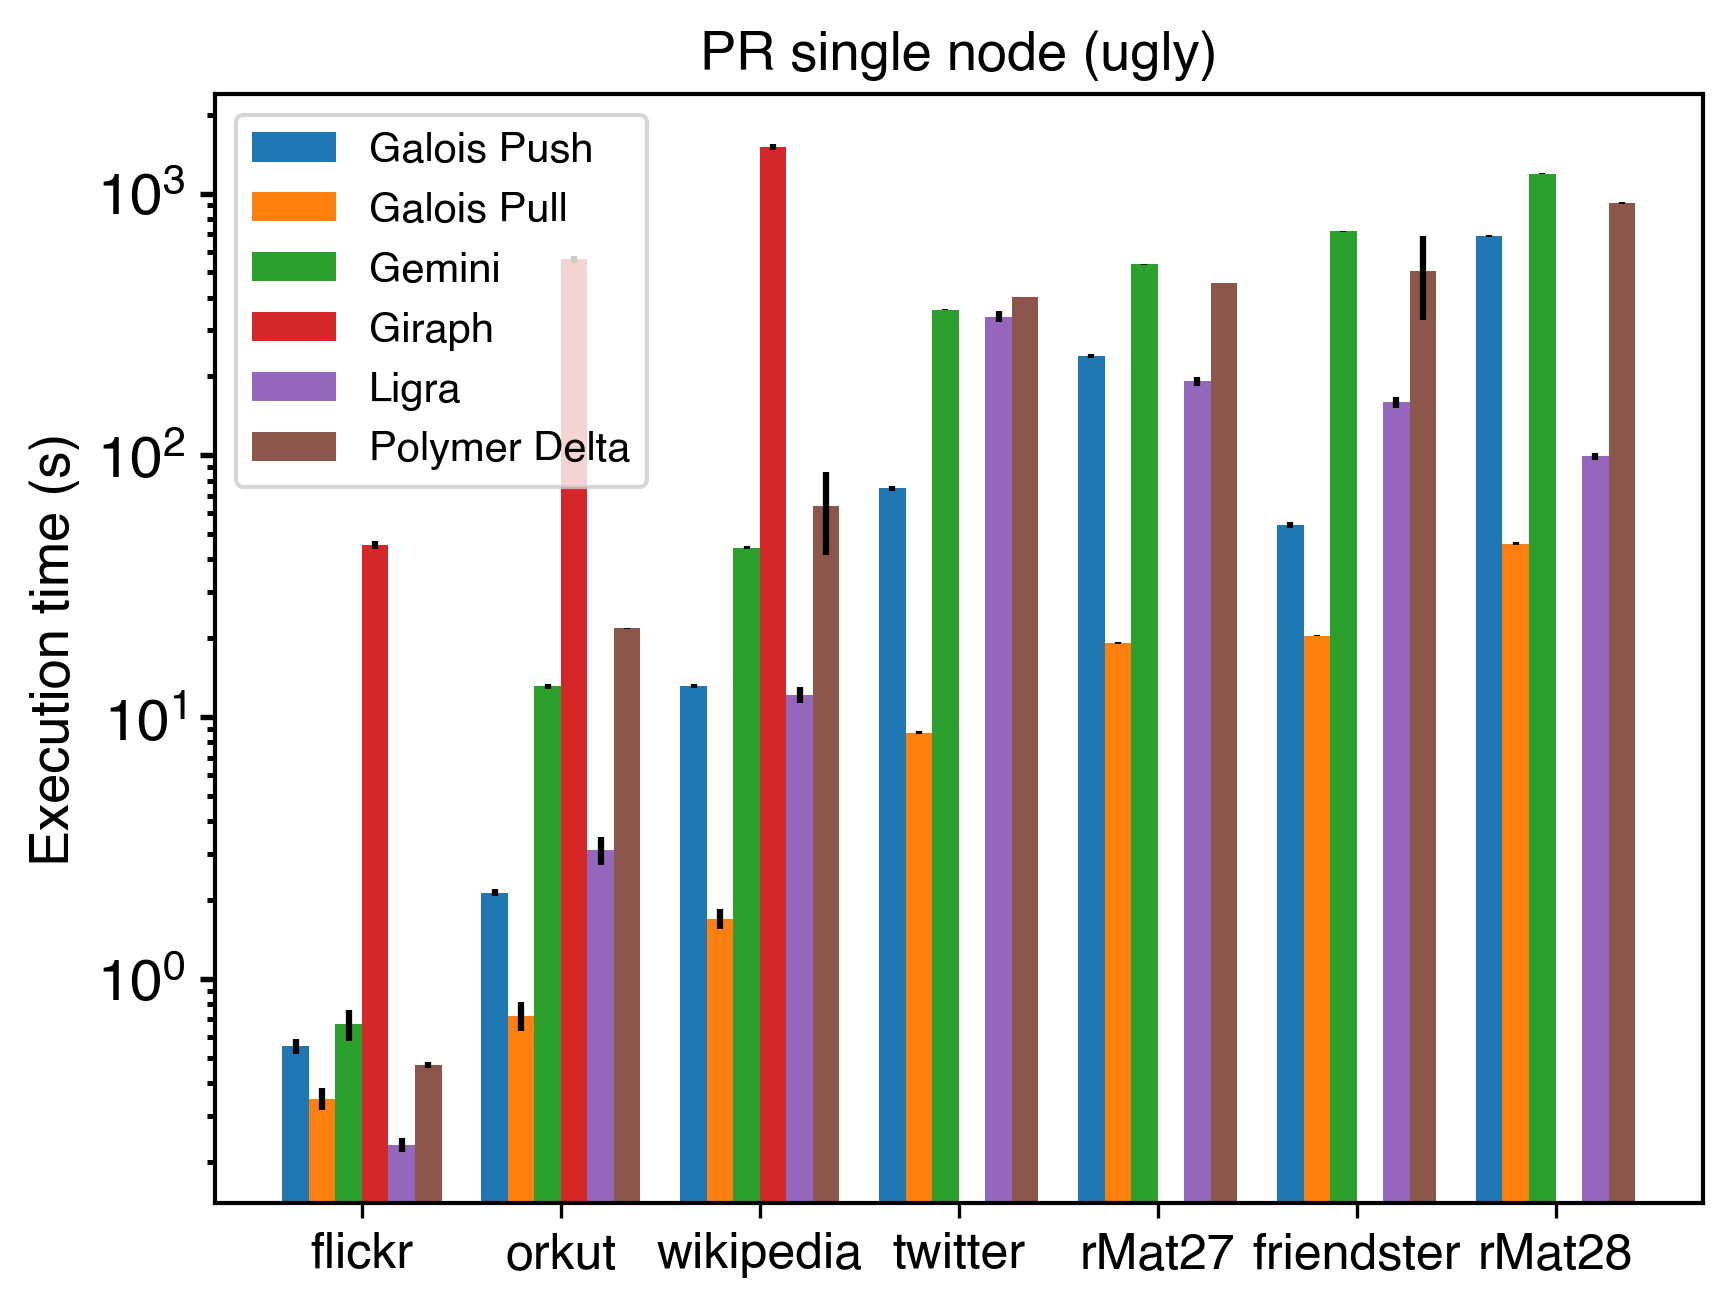
\includegraphics[width=\linewidth]{../../plots/singleNodePR_execTime.png}
		\caption{Execution time}
		\label{fig:singleNodePR_exec}
	\end{subfigure}
	\hfil
	\begin{subfigure}{0.32\textwidth}
		\includegraphics[width=\linewidth]{../../plots/singleNodePR_overheadTIme.png}
		\caption{Overhead}
		\label{fig:singleNodePR_overhead}
	\end{subfigure}
	\hfil
	\caption{Average times for PR on a single computation node, black bars represent one standard deviation in our testing}
	\label{fig:singleNodePR}
\end{figure*}

The calculation times show some odd behaviour of Galois Push. The required time is less than 1ms, regardless of the graph (cf. \autoref{fig:singleNodePR_calc}). Meanwhile there was no output produced, that would indicate any kind of error. These results would make the calculation times of Galois Push the smallest on all graphs, with a difference of at least one order of magnitude. However, we are very suspicious of these results and thus exclude the calculation time for Galois Push in further comparisons. Because the execution time of Galois Push is always considerably longer than the execution time of Galois Pull (cf. \autoref{fig:singleNodePR_calc}). This leads us to believe that the output that we used for our measurements contains an error.

For the three graphs on which Giraph computed successfully, it is the slowest framework in both calculation and execution times. And that by a difference of three orders of magnitude in the calculation time and one to two orders of magnitude in execution time (cf \autoref{fig:singleNodePR}). On the larger graphs (i.e. those, where there is no data for Giraph), Gemini and Ligra are always slowest in execution time.
Contrary to this, Galois Pull has the smallest execution times on all graphs except flickr (cf. \autoref{fig:singleNodePR_exec}). Ligra is fastest on flickr, while being second fastest on wikipedia, rMat27 and rMat28. Galois Push is second fastest on orkut and friendster.
Interestingly, the execution time for Ligra is at a maximum for twitter. The required time is steadily decreasing with increasing graph size.



\paragraph{Distributed}
\begin{figure*}
	\hfil
	\begin{subfigure}{0.32\textwidth}
		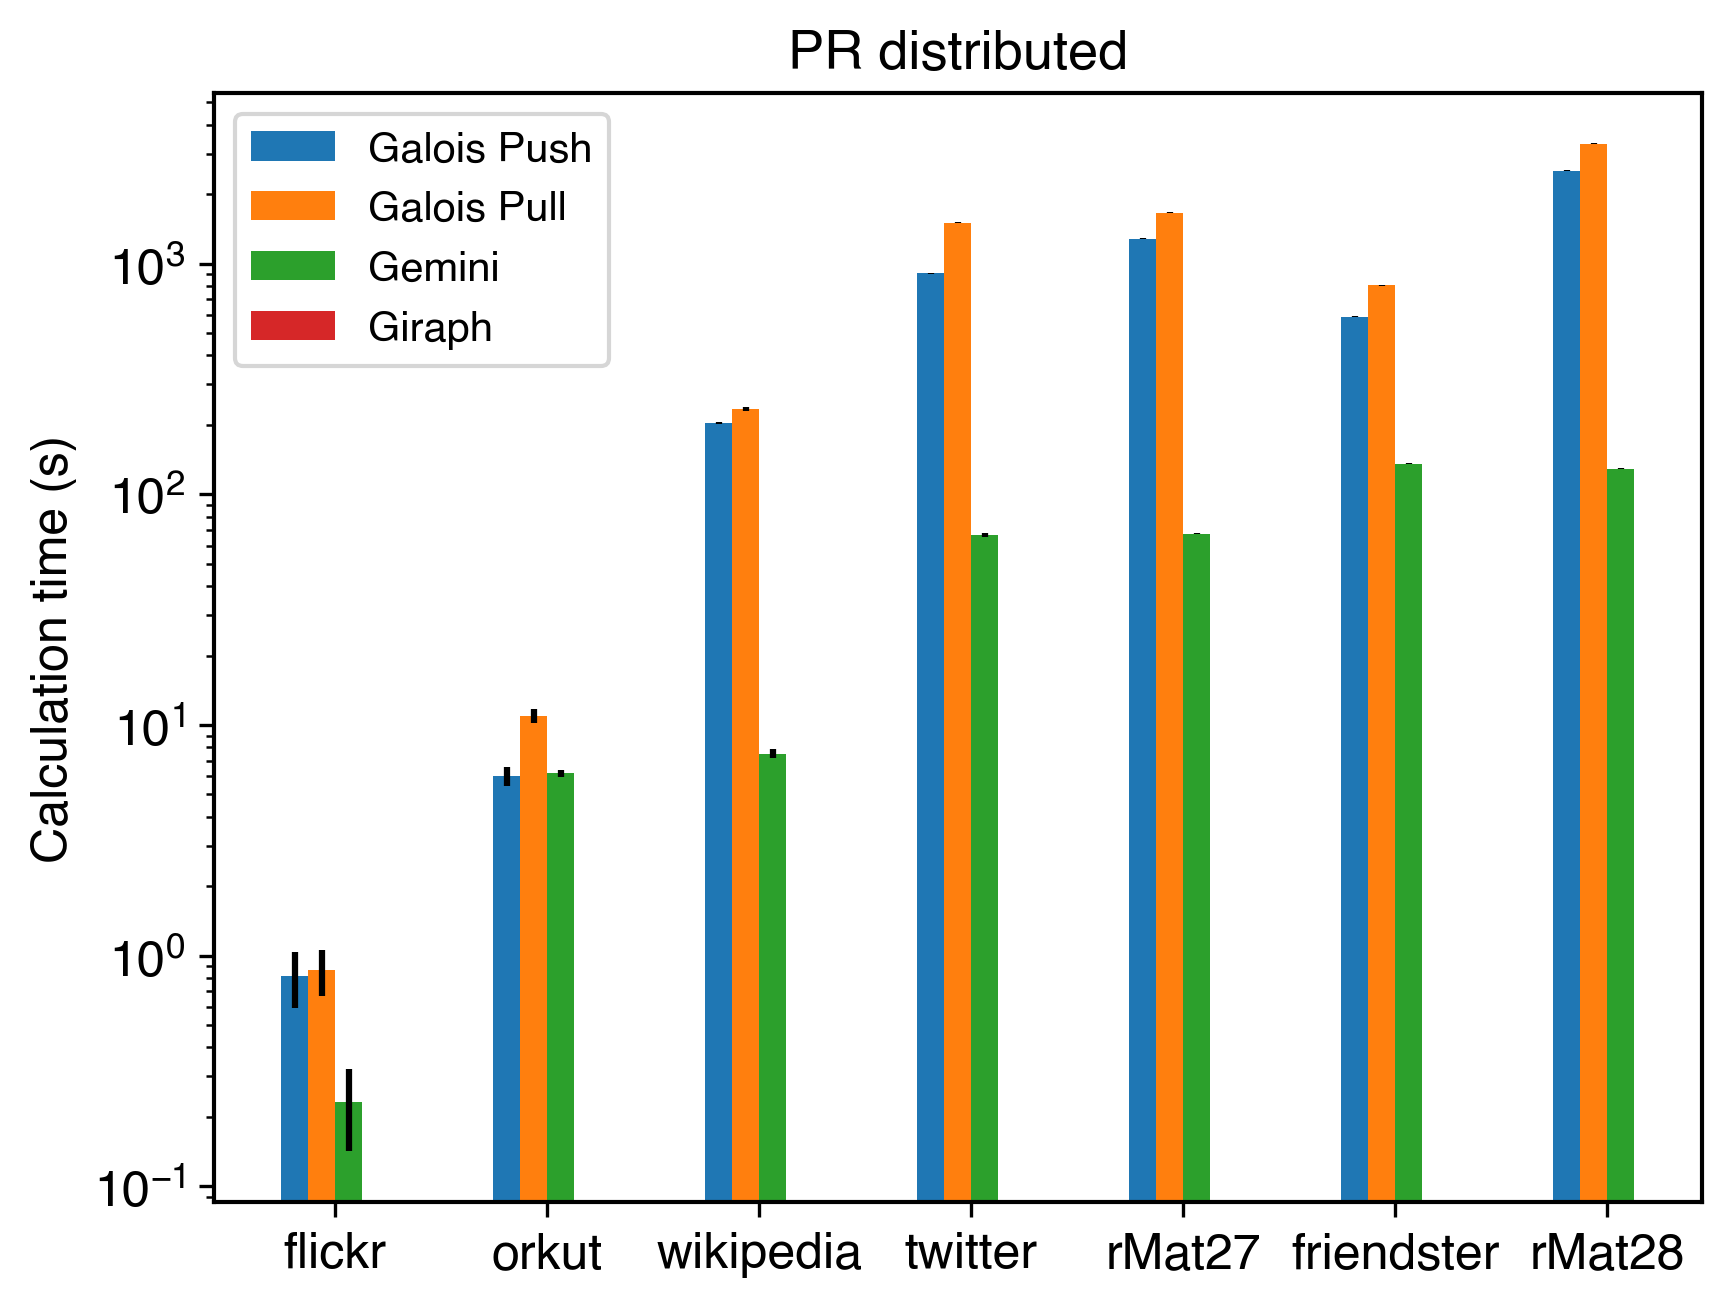
\includegraphics[width=\linewidth]{../../plots/distributedPR_calcTime.png}
		\caption{Calculation time}
		\label{fig:distributedPR_calc}
	\end{subfigure}
	\hfil
	\begin{subfigure}{0.32\textwidth}
		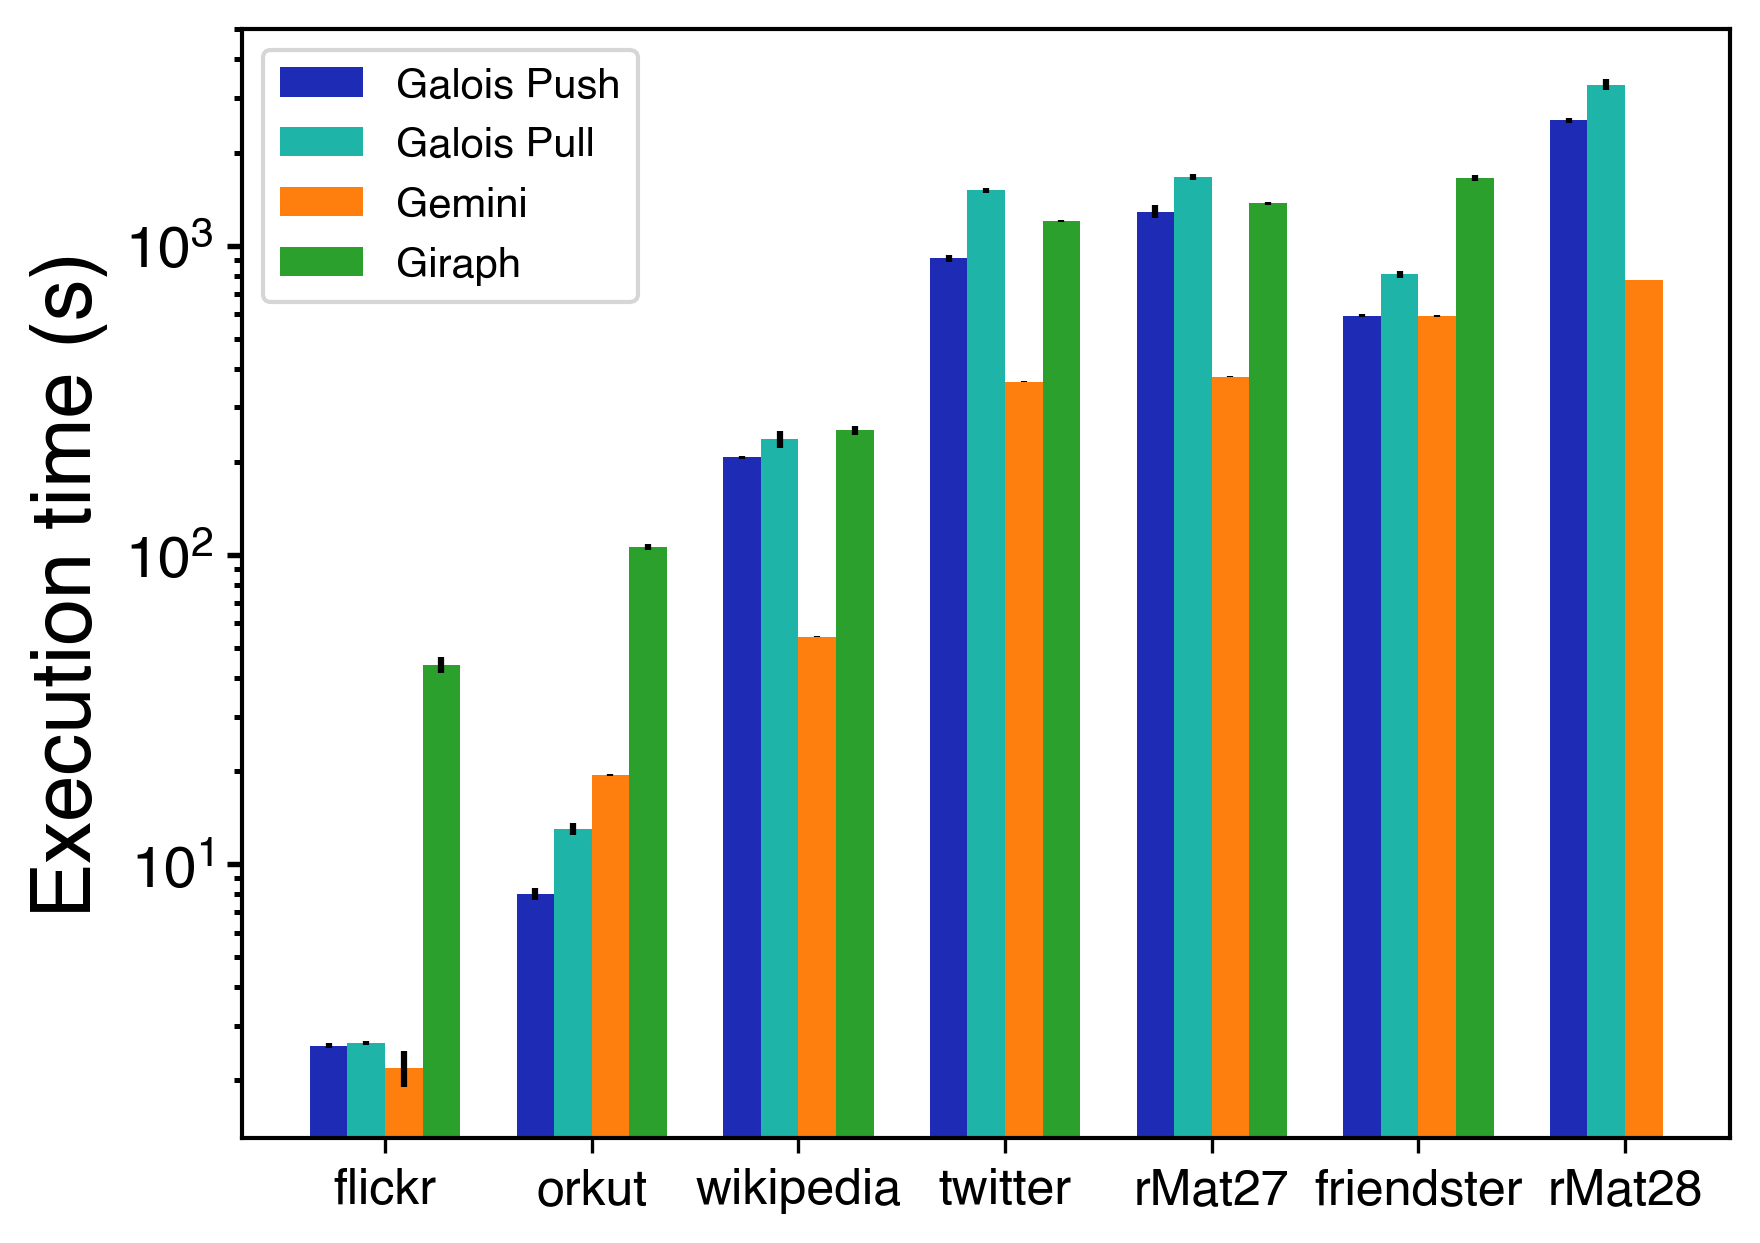
\includegraphics[width=\linewidth]{../../plots/distributedPR_execTime.png}
		\caption{Execution time}
		\label{fig:distributedPR_exec}
	\end{subfigure}
	\hfil
	\begin{subfigure}{0.32\textwidth}
		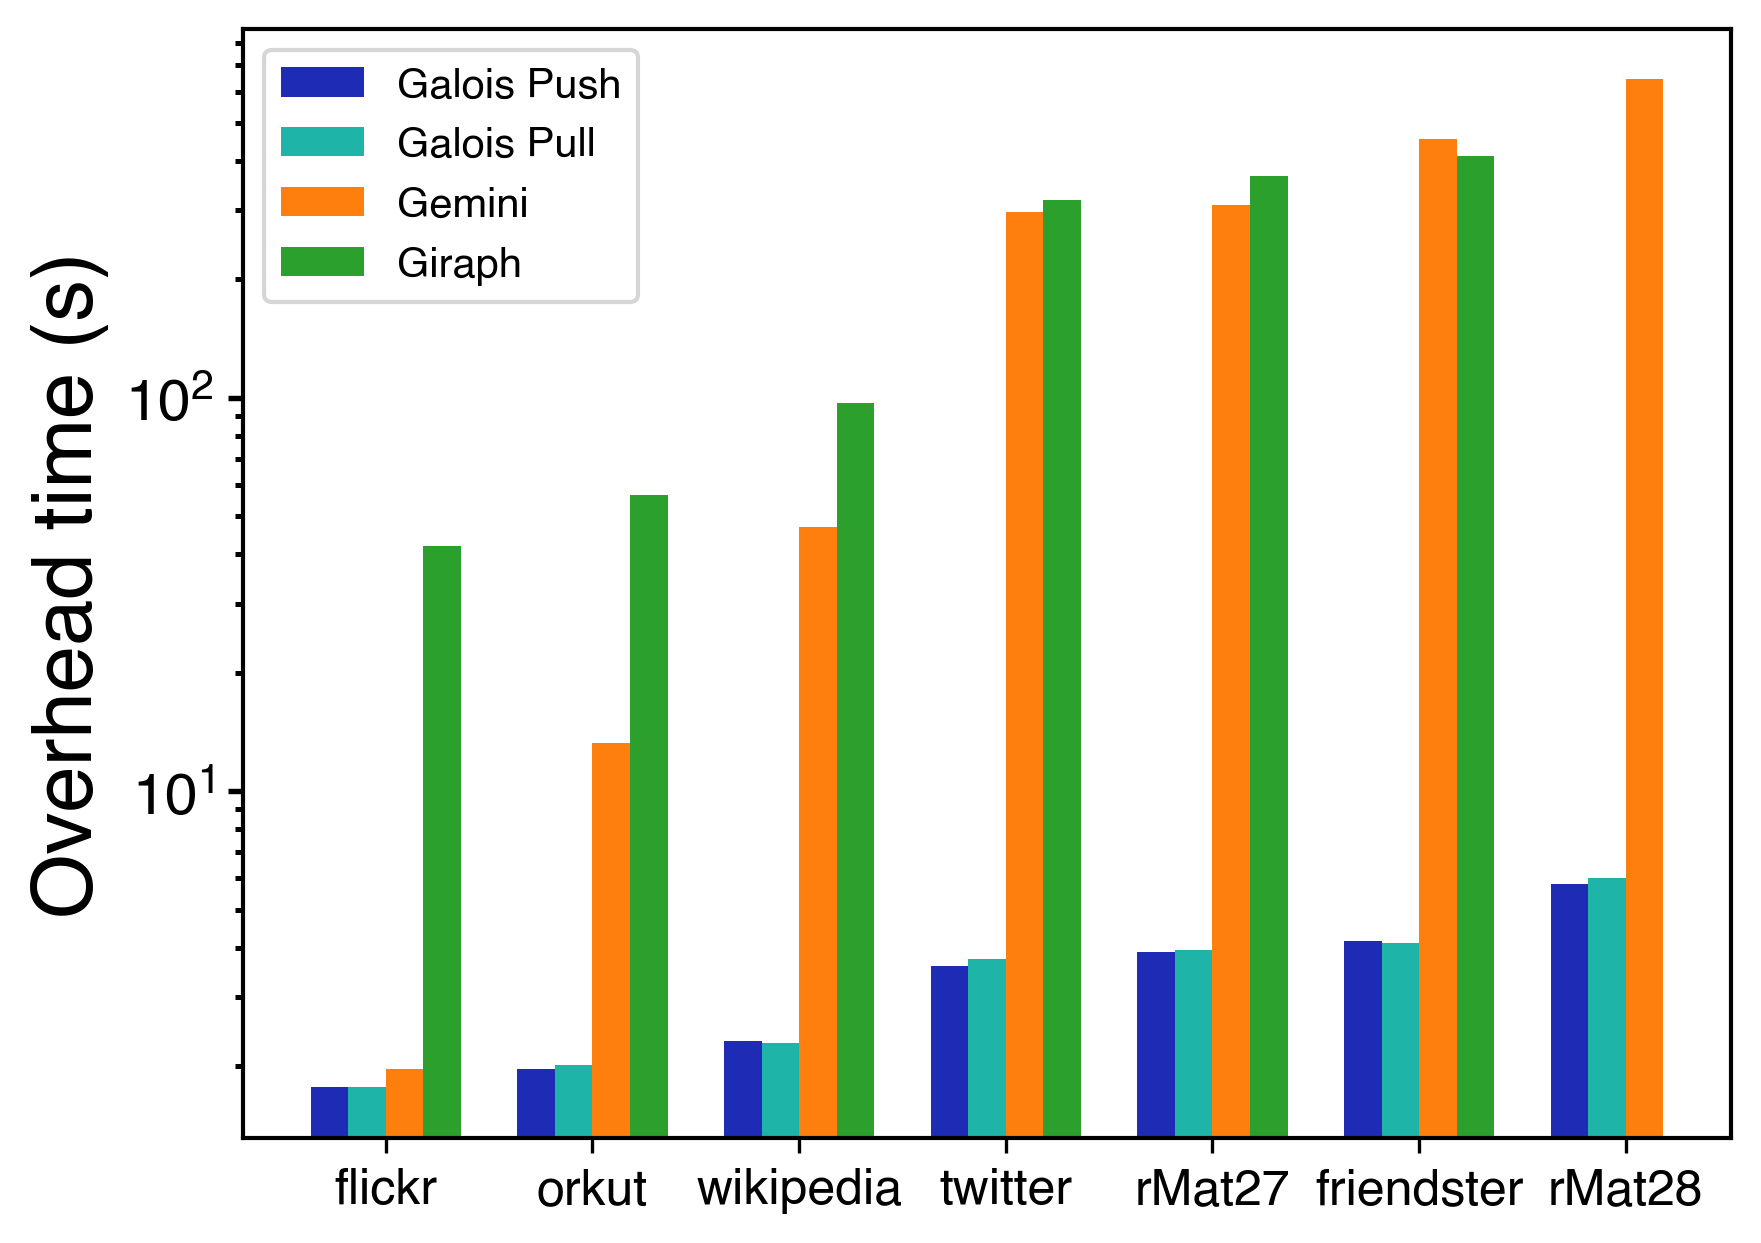
\includegraphics[width=\linewidth]{../../plots/distributedPR_overheadTime.png}
		\caption{Overhead}
		\label{fig:distributedPR_overhead}
	\end{subfigure}
	\hfil
	\caption{Average times for PR on the distributed cluster, black bars represent one standard deviation in our testing}
	\label{fig:distributedPR}
\end{figure*}

Our benchmark results of PageRank on the distributed cluster can be seen in \autoref{fig:distributedPR}.
First of all, Giraph was unable to complete the test on rMat28 because it ran out of memory, thus this result is missing.
When comparing the calculation times in \autoref{fig:distributedPR_calc} to the execution times in \autoref{fig:distributedPR_exec}, we see similar behaviour of all frameworks.
This means that unlike with SSSP or BFS, the calculation times and execution times are similar with respect to the relations of the frameworks to one another.

Gemini has the shortest calculation times on all graphs (cf. \autoref{fig:distributedPR_calc}).
The two Galois implementations are second on flickr, orkut, friendster and rMat28, with Giraph being second on the others.
Generally, the calculation of Galois Push is anywhere from 6\% (flickr) to 46\% (orkut) faster than the Pull counterpart.

This applies to the execution times in almost the same way (cf. \autoref{fig:distributedPR_exec}).
Gemini is the fastest on all graphs except orkut, where both Galois implementations are faster. Galois Pull takes 13s, whereas Gemini requires 19.4s on orkut.
Again, as for the calculation times, Galois is the second fastest framework on flickr, wikipedia, friendster and rMat28.
And Galois Push has smaller execution times than the Pull version because the overhead times for both implementations are similar (cf. \autoref{fig:distributedPR_overhead}).



%!TEX root=../../main.tex




\subsection{Galois speedup}
\label{sec:galois_speedup}
Analyzing the calculation time speedups for Galois, we can compare how or if the different algorithms benefit from increasing thread numbers.


\begin{figure*}
	\hfil
	\begin{subfigure}{0.32\textwidth}
		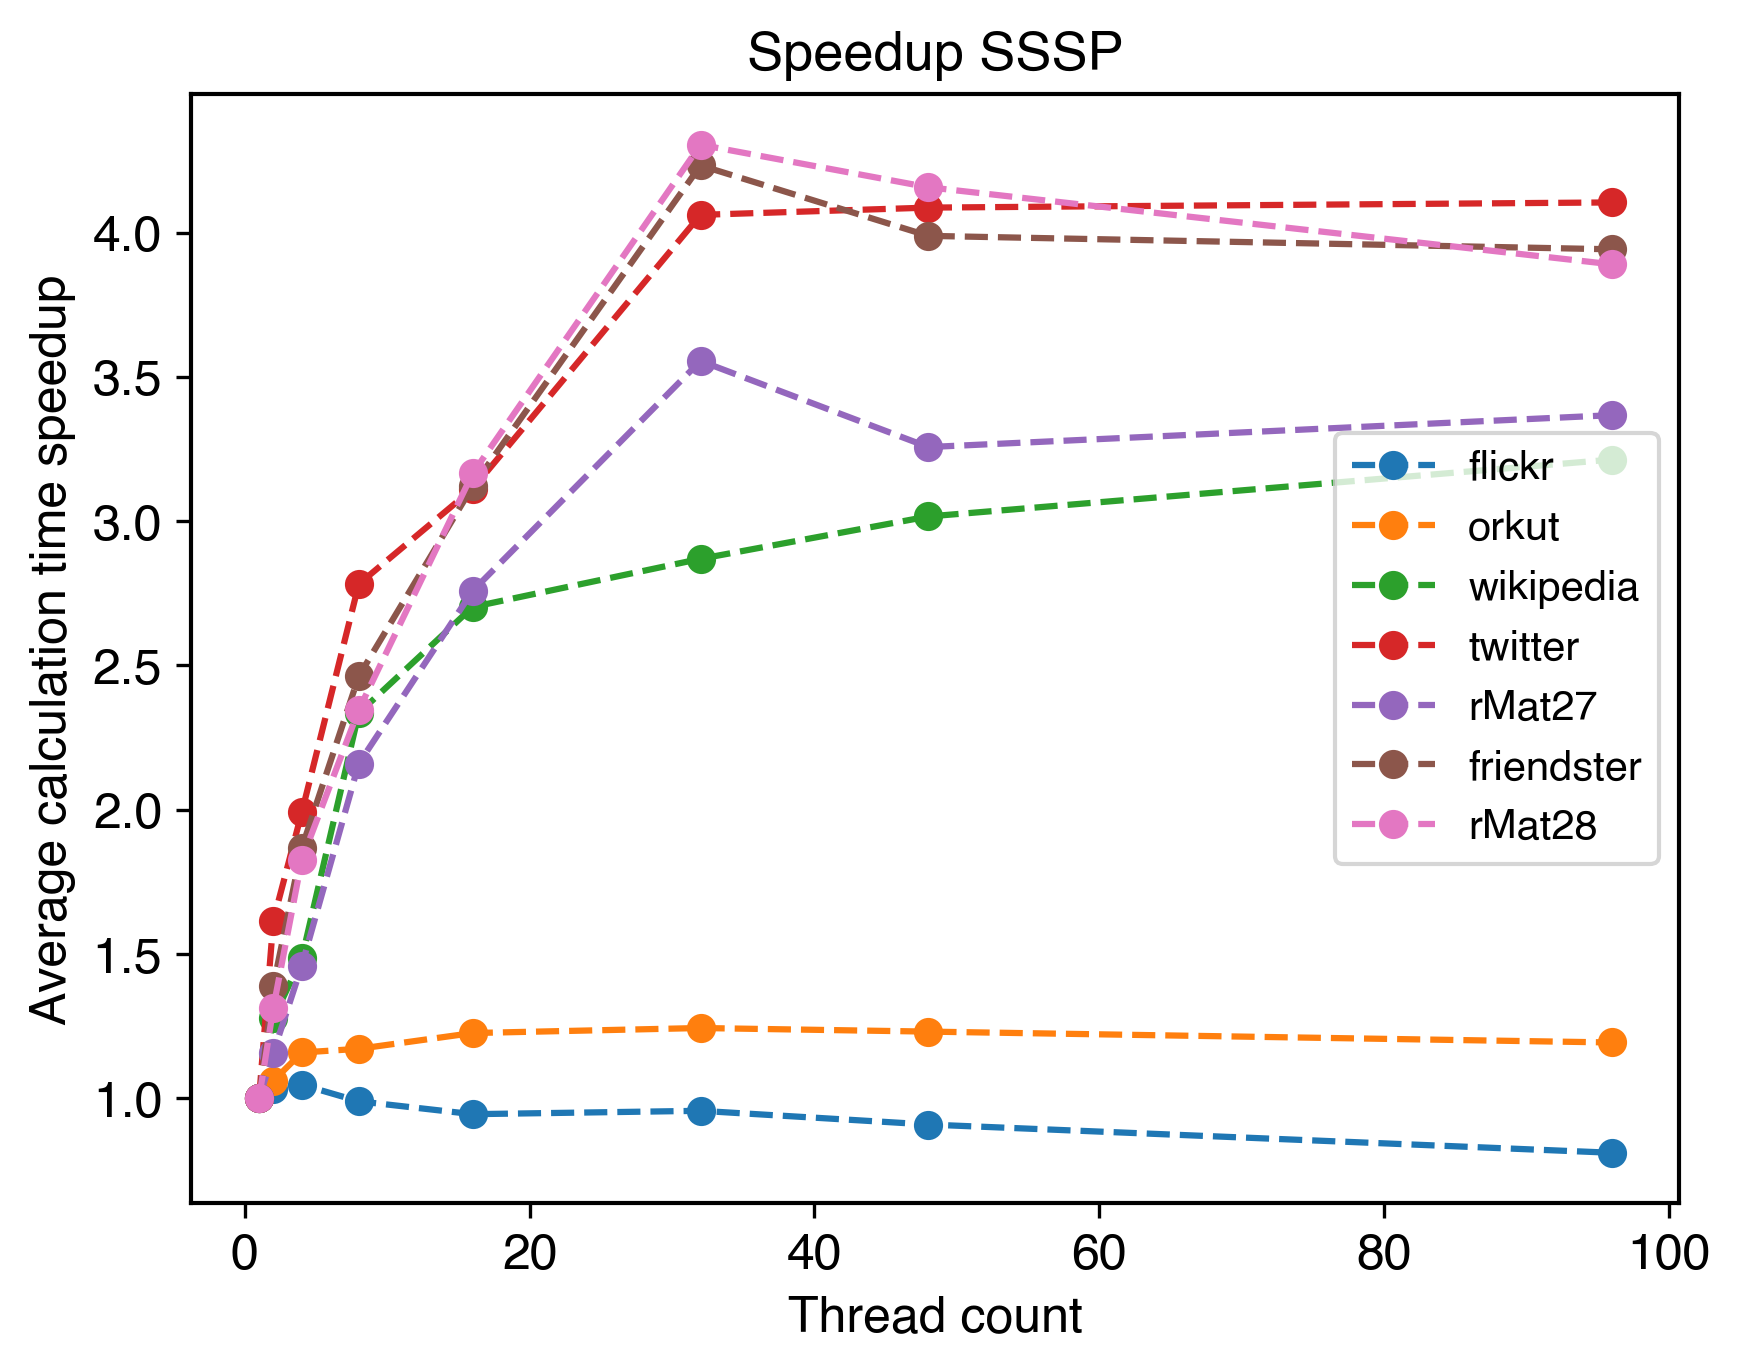
\includegraphics[width=\linewidth]{../../plots/singleNodeSSSPGaloisThreads.png}
		\caption{Calculation time speedup with increasing thread count for Galois Single-source Shortest-paths}
		\label{fig:galoisSpeedupSSSP}
	\end{subfigure}
	\hfil
	\begin{subfigure}{0.32\textwidth}
		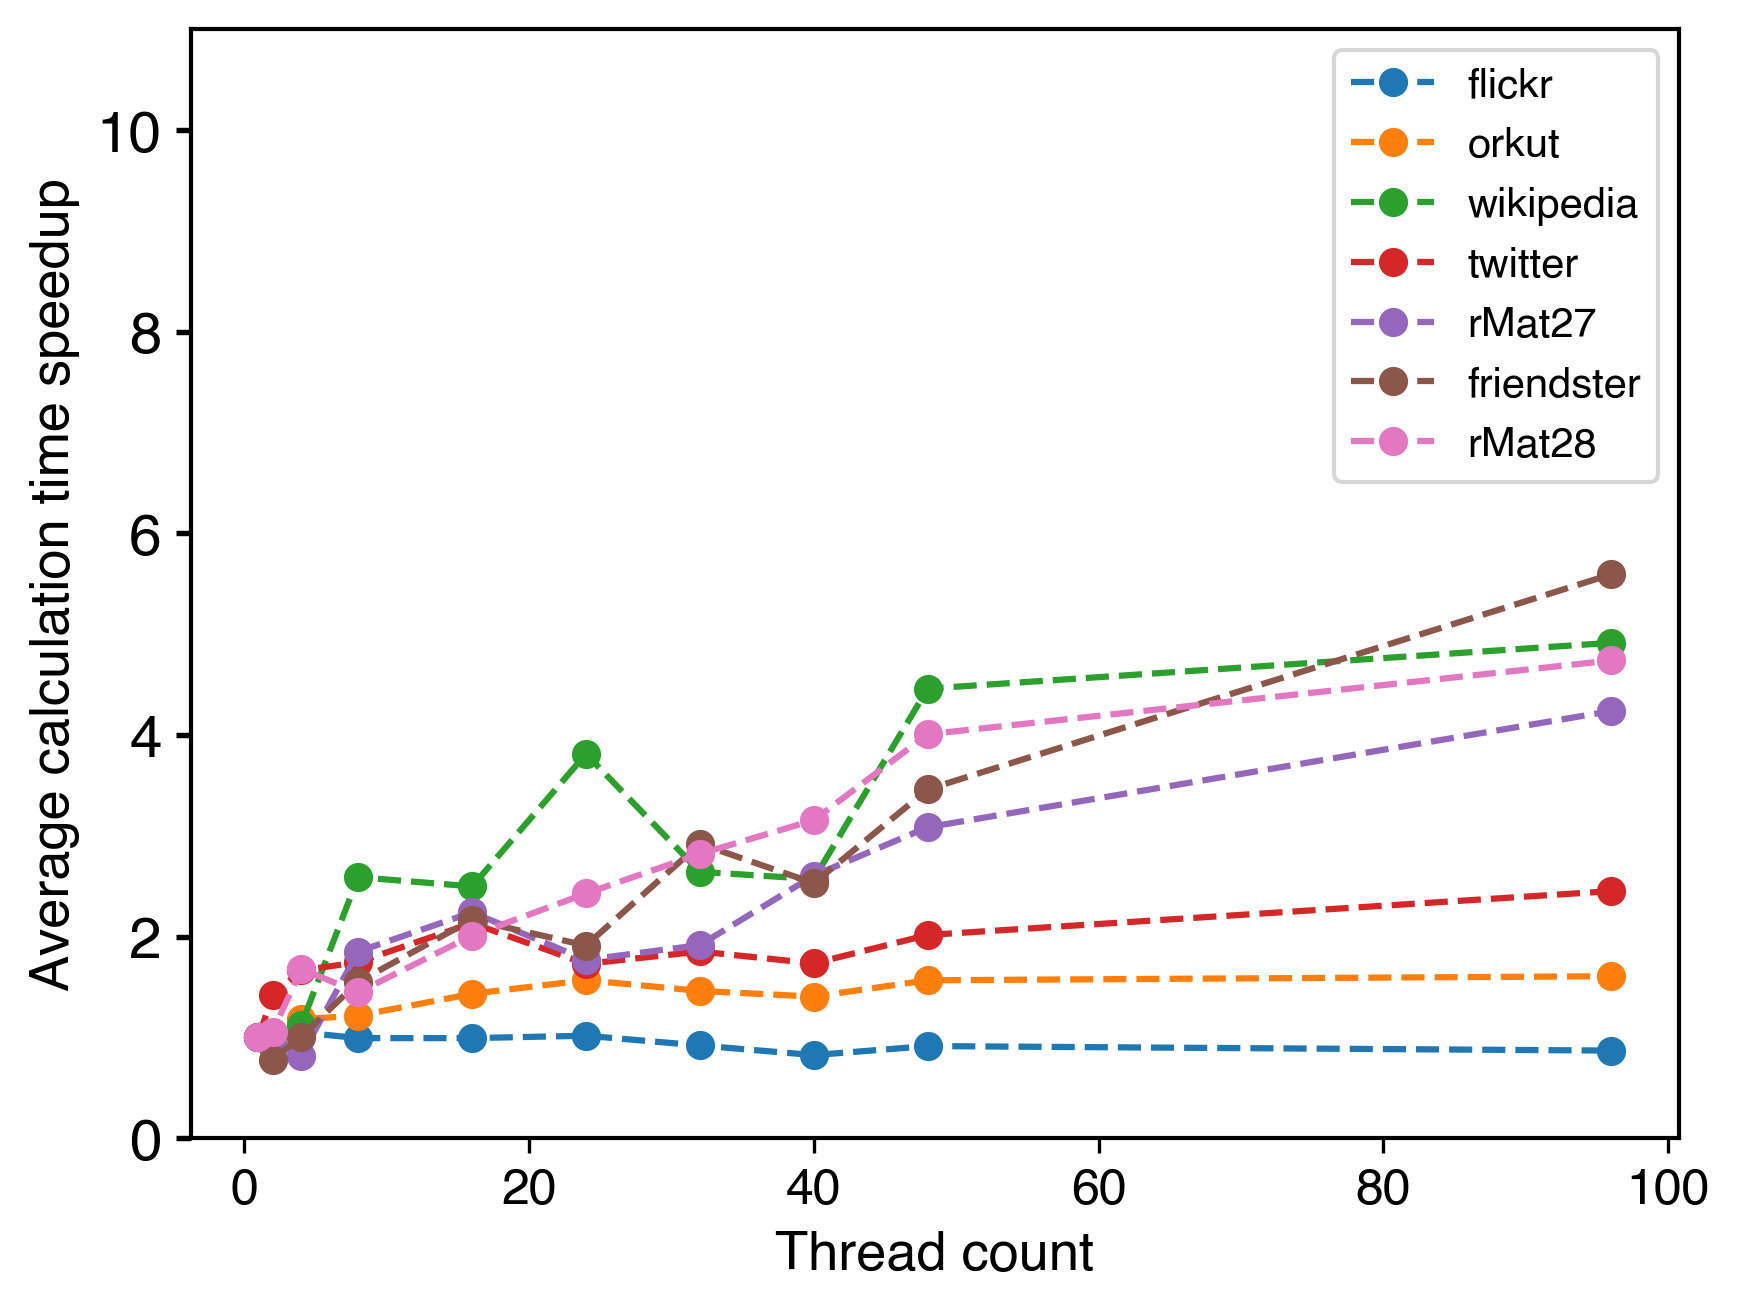
\includegraphics[width=\linewidth]{../../plots/singleNodeBFSGaloisThreads.png}
		\caption{Calculation time speedup with increasing thread count for Galois Breadth-first search}
		\label{fig:galoisSpeedupBFS}
	\end{subfigure}
	\hfil
\end{figure*}



\subsubsection{Single-source Shortest-path}

Starting with SSSP, we see an algorithm that benefits from many available threads in \autoref{fig:galoisSpeedupSSSP}.
For all larger graphs, speedup is in most cases very close to optimal up to about 8 threads.
Twitter has the best speedup overall. It is 2.6$\times$ with 2 threads compared to one, 4$\times$ with 4, 7.7$\times$ with 8 and 9.7$\times$ using 16 threads.
Behaviour on friendster is similarly good. Here speedup is 1.9$\times$ at 2 threads compared to one, 3.5$\times$ at 4, 6.1$\times$ at 8 threads and 9.7$\times$ at 16 threads.
Anything above 16 threads however no longer helps decrease the computation time significantly on any graph. Speedup above 16 threads is always less than double the speedup of 16 threads. The maximum measured speedups are 10$\times$ (96 threads) for wikipedia, 17$\times$ (96 threads) for twitter, 11$\times$ (96 threads) for rMat27, 16$\times$ (48 threads) for friendster and 19$\times$ (40 threads) for rMat28.
In some cases increasing thread counts even prolongues calculation time. For example calculation on rMat28 is actually slower with 48 or 96 threads compared to 40 threads. For 40 threads, the speedup is nearly 19$\times$, on 48 threads 17$\times$ and with 96 threads only 15$\times$ compared to one thread.

Small graphs, i.e. flickr and orkut neither benefit from more threads nor is the performance significantly held up by synchronization overhead.
Performance on flickr can not be sped up at all, with speedup on flickr being very close to 1 for 1 to 8 threads and between 0.7$\times$ to 0.9$\times$ from 16 to 96 threads.
Orkut reaches maximum speedup of 1.6$\times$ at 16 threads. However on orkut, the speedup is always greater or equal to 1.


\subsubsection{Breadth-first search}


For our speedup results on BFS, \autoref{fig:galoisSpeedupBFS} shows the calculation time speedup of Galois' BFS.
On all graphs, the speedup never exceeds 6$\times$ even when using 96 threads.
For the smaller graphs (flickr, orkut), we have the same behaviour as on SSSP. Speedup is close to 1 in all cases, with orkut reaching a maximum speedup of 1.6$\times$ at 24 threads.
On the larger graphs, speedup is possible but only to a very small degree.
Wikipedia has a maximum speedup of 4.9$\times$ at 96 threads, for twitter it is 2.5$\times$ at 96 threads and 5.6$\times$ on friendster. The two synthetic data sets reach speedups of 4.2$\times$ and 4.7$\times$ for rMat27 and rMat28 on 96 threads.


\subsubsection{PageRank}
We want to first take a look at the results for PageRank in Pull mode, seen in \autoref{fig:galoisSpeedupPRPull}. This is a perfect example for an algorithm that does not benefit from multithreaded computation.
Computation is hardly sped up on any graph other than flicker, where the reached maximum is 64\%. This maximum is reached at two threads, with speedup steadily declining above that.
The rMat28 is the only other graph of one could say computation was sped up at large thread counts. Here we reached a maximum speedup of 31\%\ at 96 threads.
All 5 other graphs only reach a speedup greater or equal to 1 in just one or two cases and if so only by a small margin.
Computation on Orkut and Twitter reaches a speedup maximum of 12\%\ and 5\%\ at 4 threads, while being less or equal to 1 in all other cases.
The wikipedia graph is never sped up.
Friendster and rMat27 can be sped up by 6.5\%\ or 10\%\ respectively on 8 threads.

Speedup results on PageRank show odd behaviour in the Galois implementation.
There is a significant performance loss on 4, 24 and 40 threads that is far from the expected behaviour. This is most visible for the Push variant seen in \autoref{fig:galoisSpeedupPRPush}, we validated the shown results two times.
Especially, the speedup for 24 threads is (by interpolating between 16 and 32 threads) expected to be anywhere between 25\% and 94\%.
Actually however, the system does not reach a speedup of more than 4\%\ on any graph, with only rMat27 actually reaching a value greater than 1.
On all other graphs, using 24 threads is anywhere from 3\% (flickr) to 9\%\ (wikipedia) slower than using just one thread.

Similar yet less pronounced behaviour is oberservable for Pull in \autoref{fig:galoisSpeedupPRPull}.
Here especially the values for 24 and 40 threads show a loss in performance.
It is most visible on the values for twitter and friendster, where both values drop significantly compared to the neighbouring 32 and 48 thread results.

\begin{figure*}
	\hfil
	\begin{subfigure}{0.32\textwidth}
		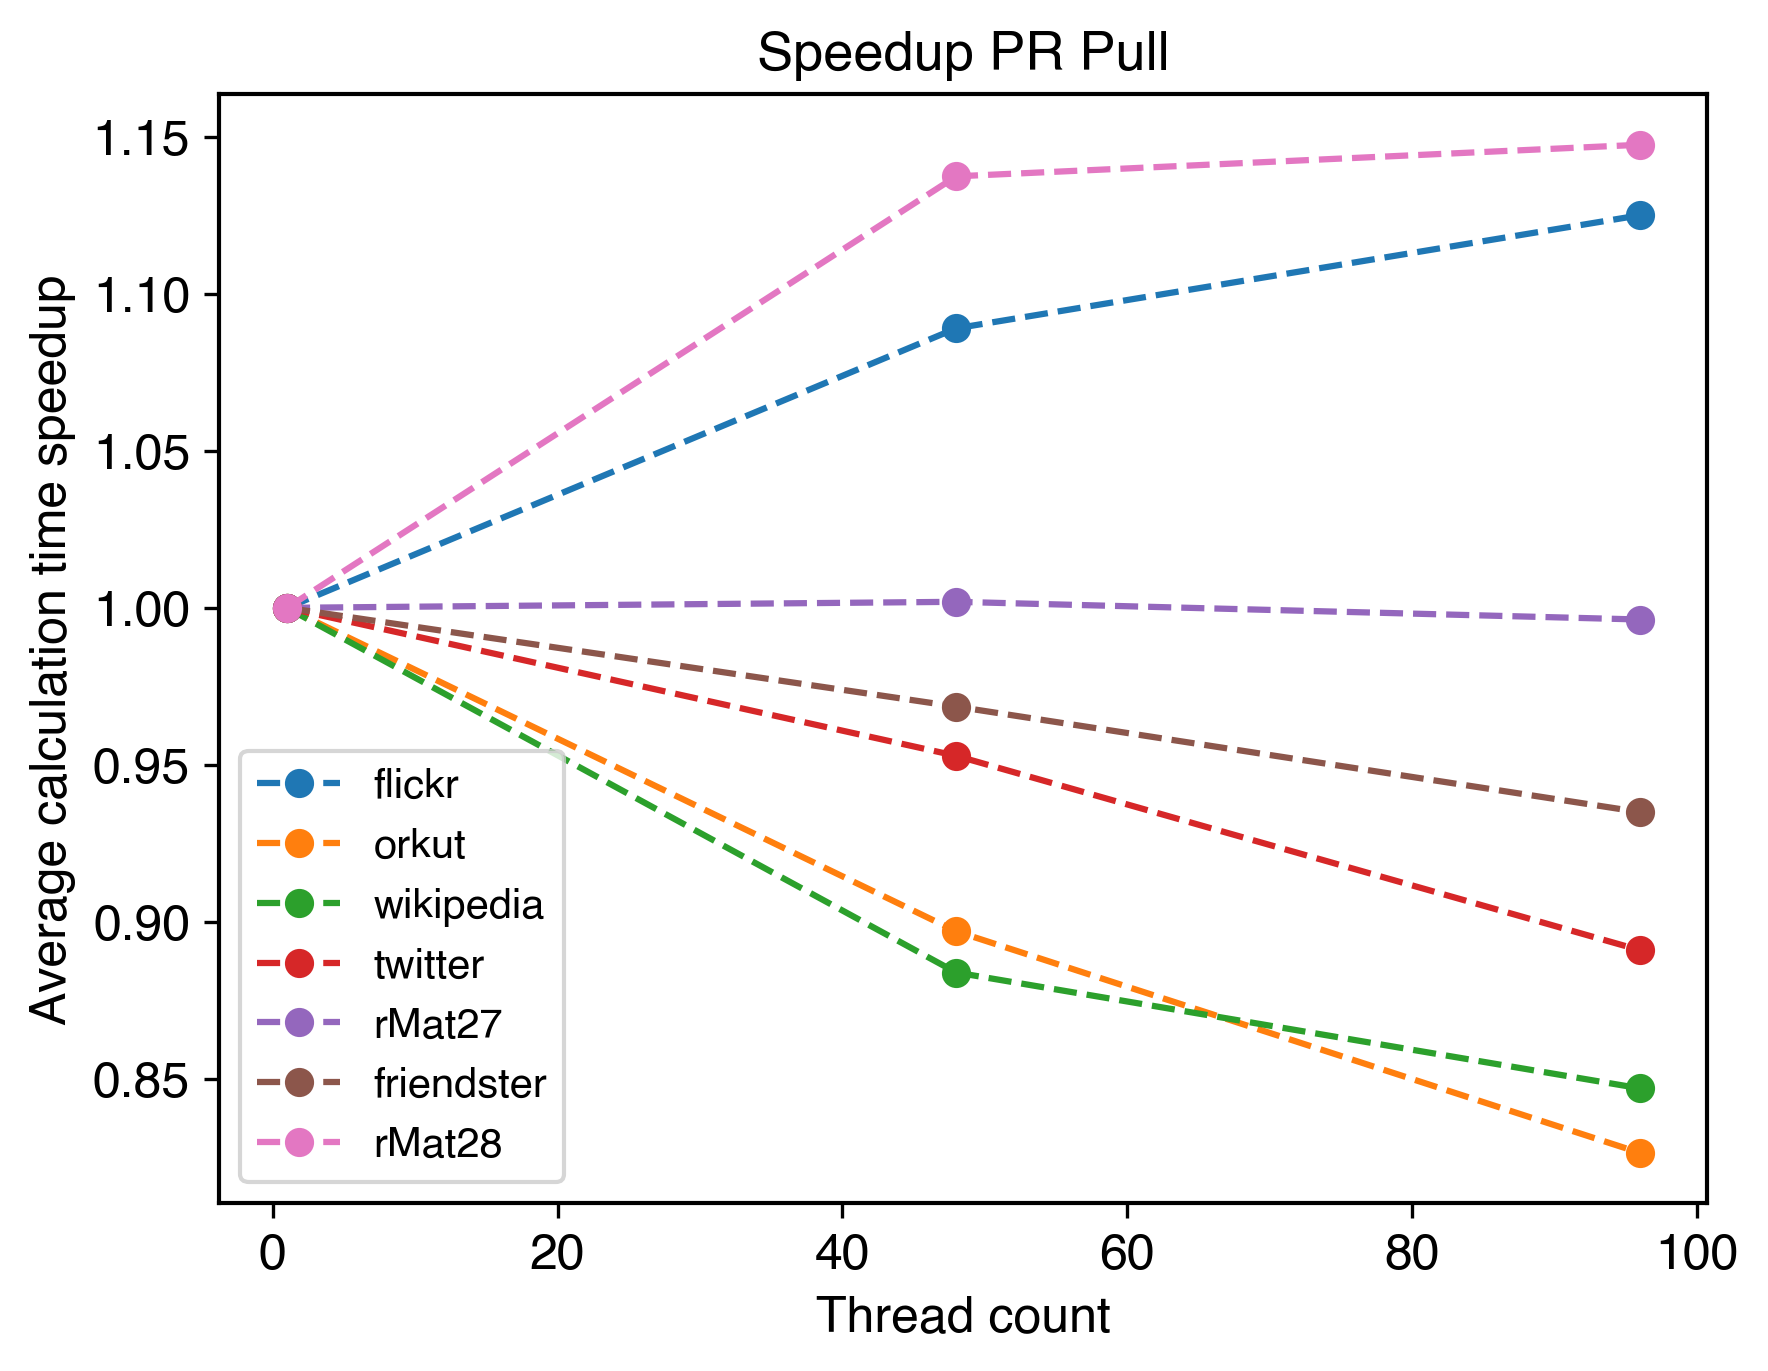
\includegraphics[width=\linewidth]{../../plots/singleNodePRPullGaloisThreads.png}
		\caption{PageRank Pull}
		\label{fig:galoisSpeedupPRPull}
	\end{subfigure}
	\hfil
	\begin{subfigure}{0.32\textwidth}
		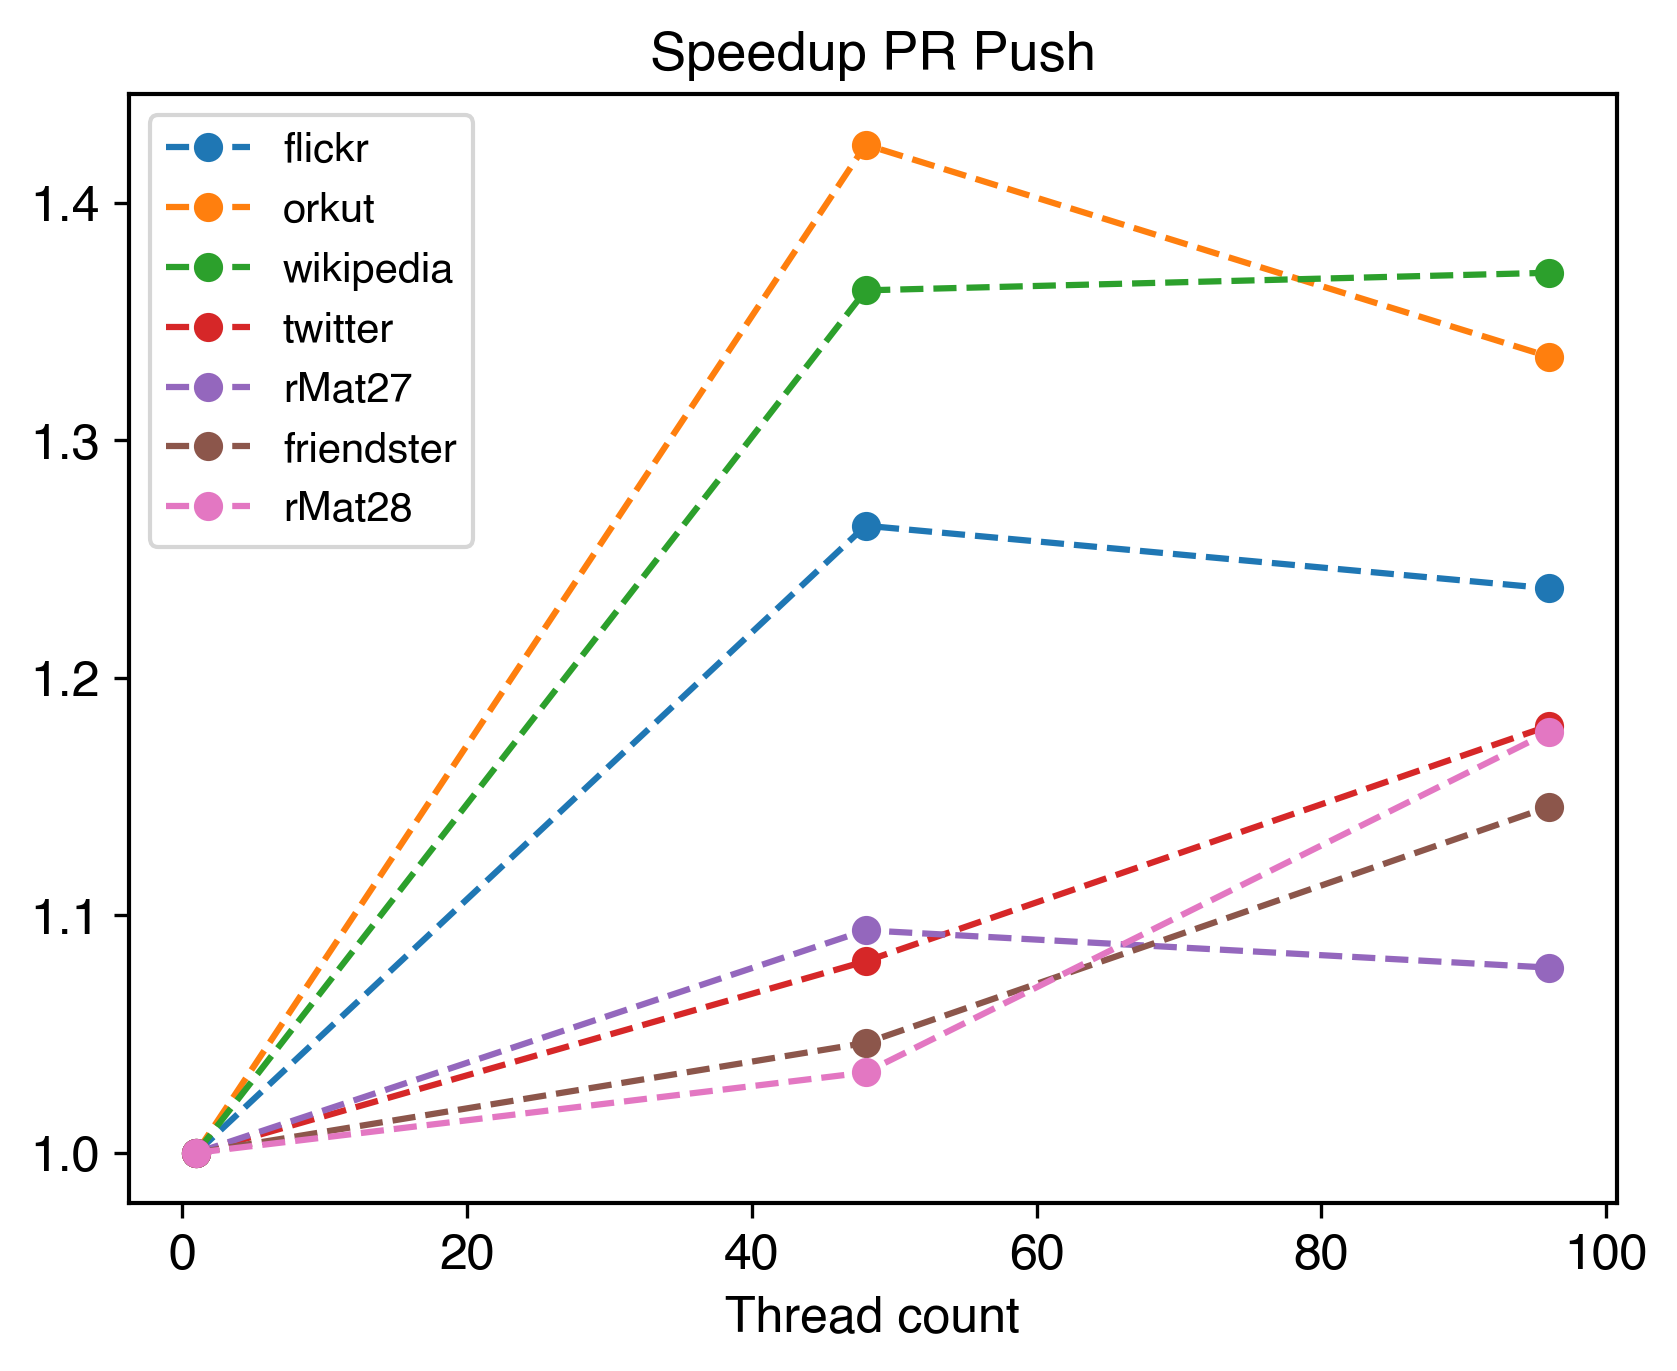
\includegraphics[width=\linewidth]{../../plots/singleNodePRPushGaloisThreads.png}
		\caption{PageRank Push}
		\label{fig:galoisSpeedupPRPush}
	\end{subfigure}
	\hfil
	\caption{Calculation time speedup with increasing thread count for Galois PageRank Push and Pull algorithms.}
\end{figure*}


\section{Hugepages}
\todo{Section}
\begin{figure}
	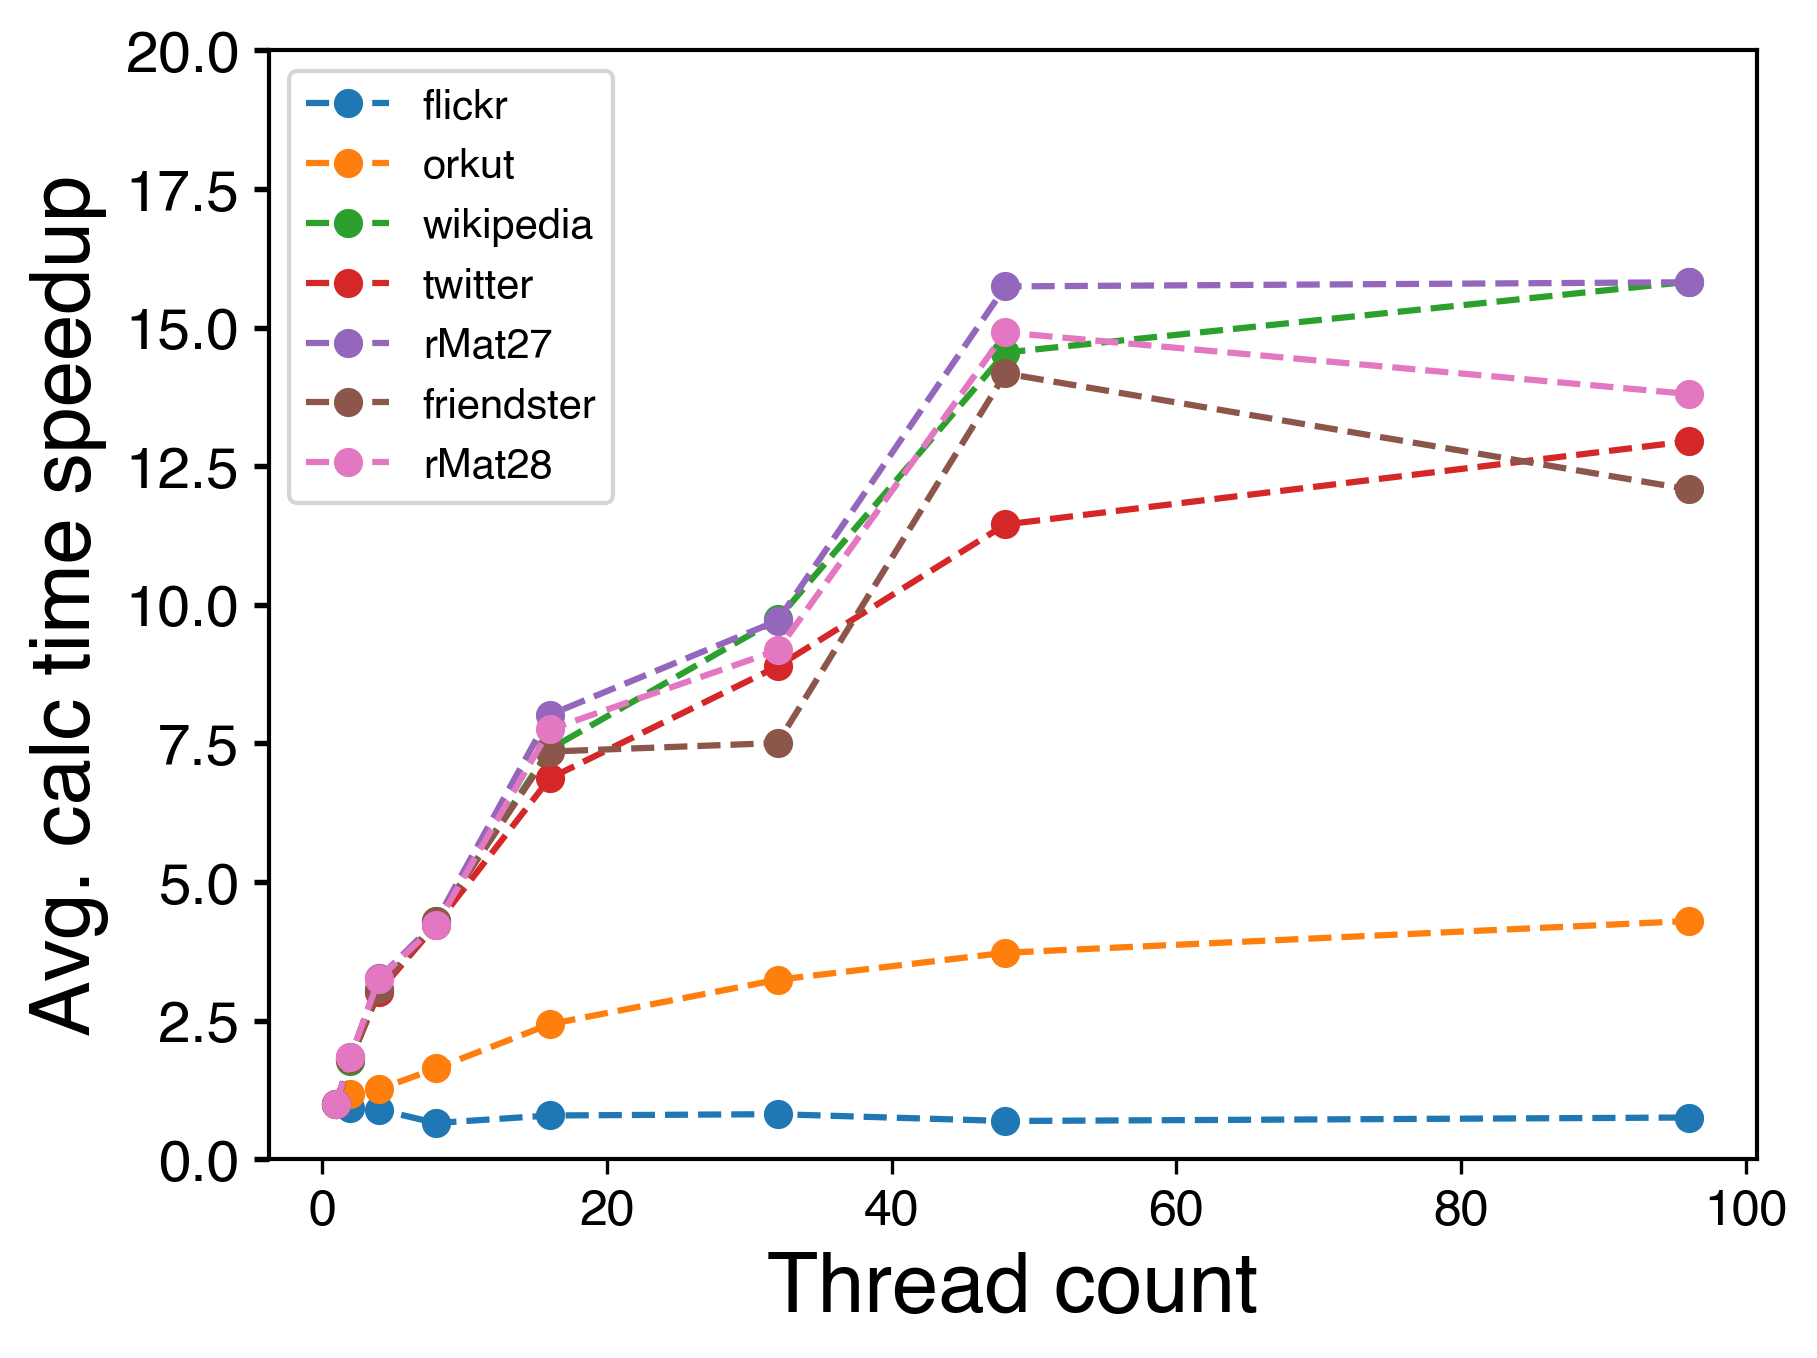
\includegraphics[width=\linewidth]{../../plots/singleNodeSSSPGaloisHPThreads.png}
	\caption{Calculation time speedup with increasing thread count for Galois Single-source Shortest-paths with Hugepages}
	\label{fig:galoisHPSpeedupSSSP}
\end{figure}

\begin{figure}
	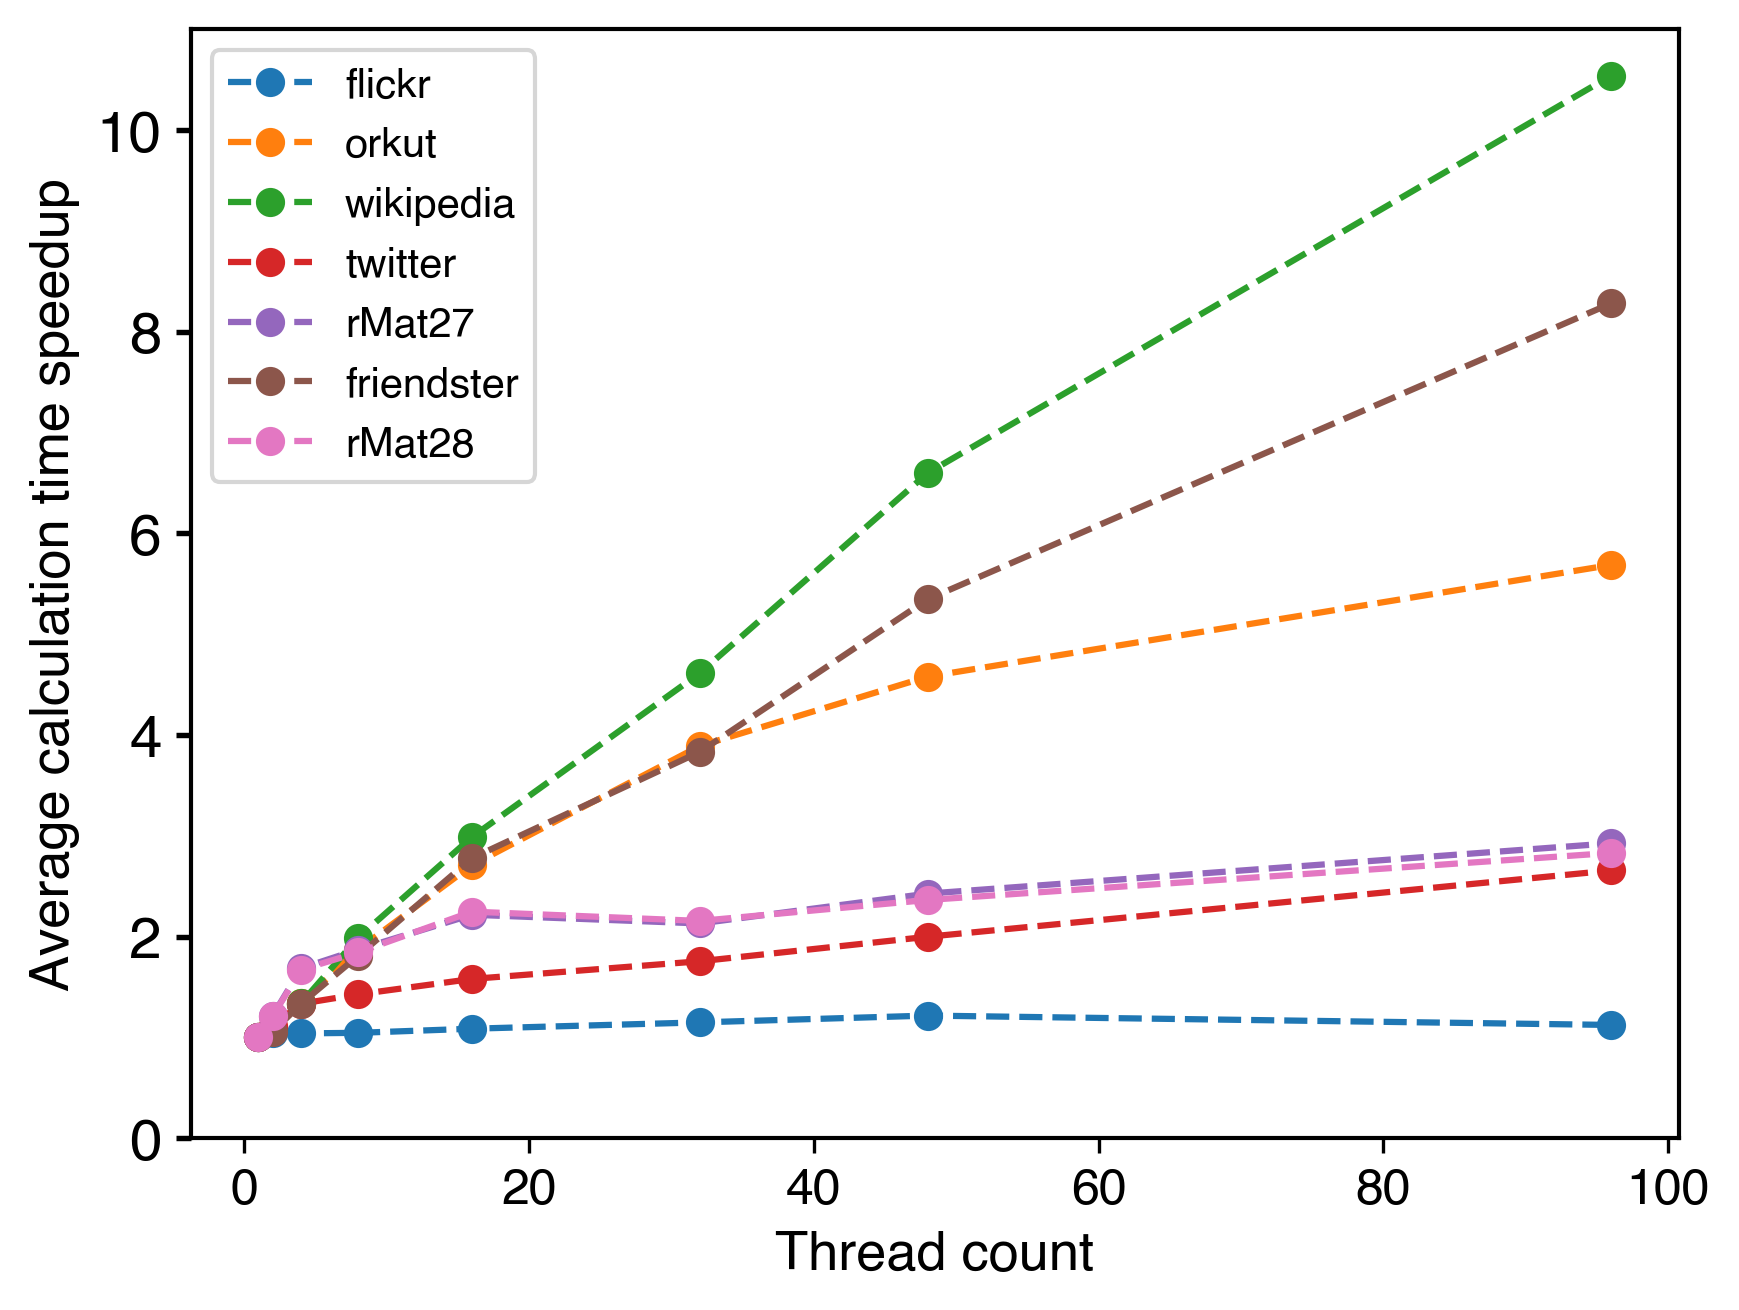
\includegraphics[width=\linewidth]{../../plots/singleNodeBFSGaloisHPThreads.png}
	\caption{Calculation time speedup with increasing thread count for Galois Breadth-first search with Hugepages}
	\label{fig:galoisHPSpeedupBFS}
\end{figure}

\begin{figure}
	\begin{subfigure}{\columnwidth}
		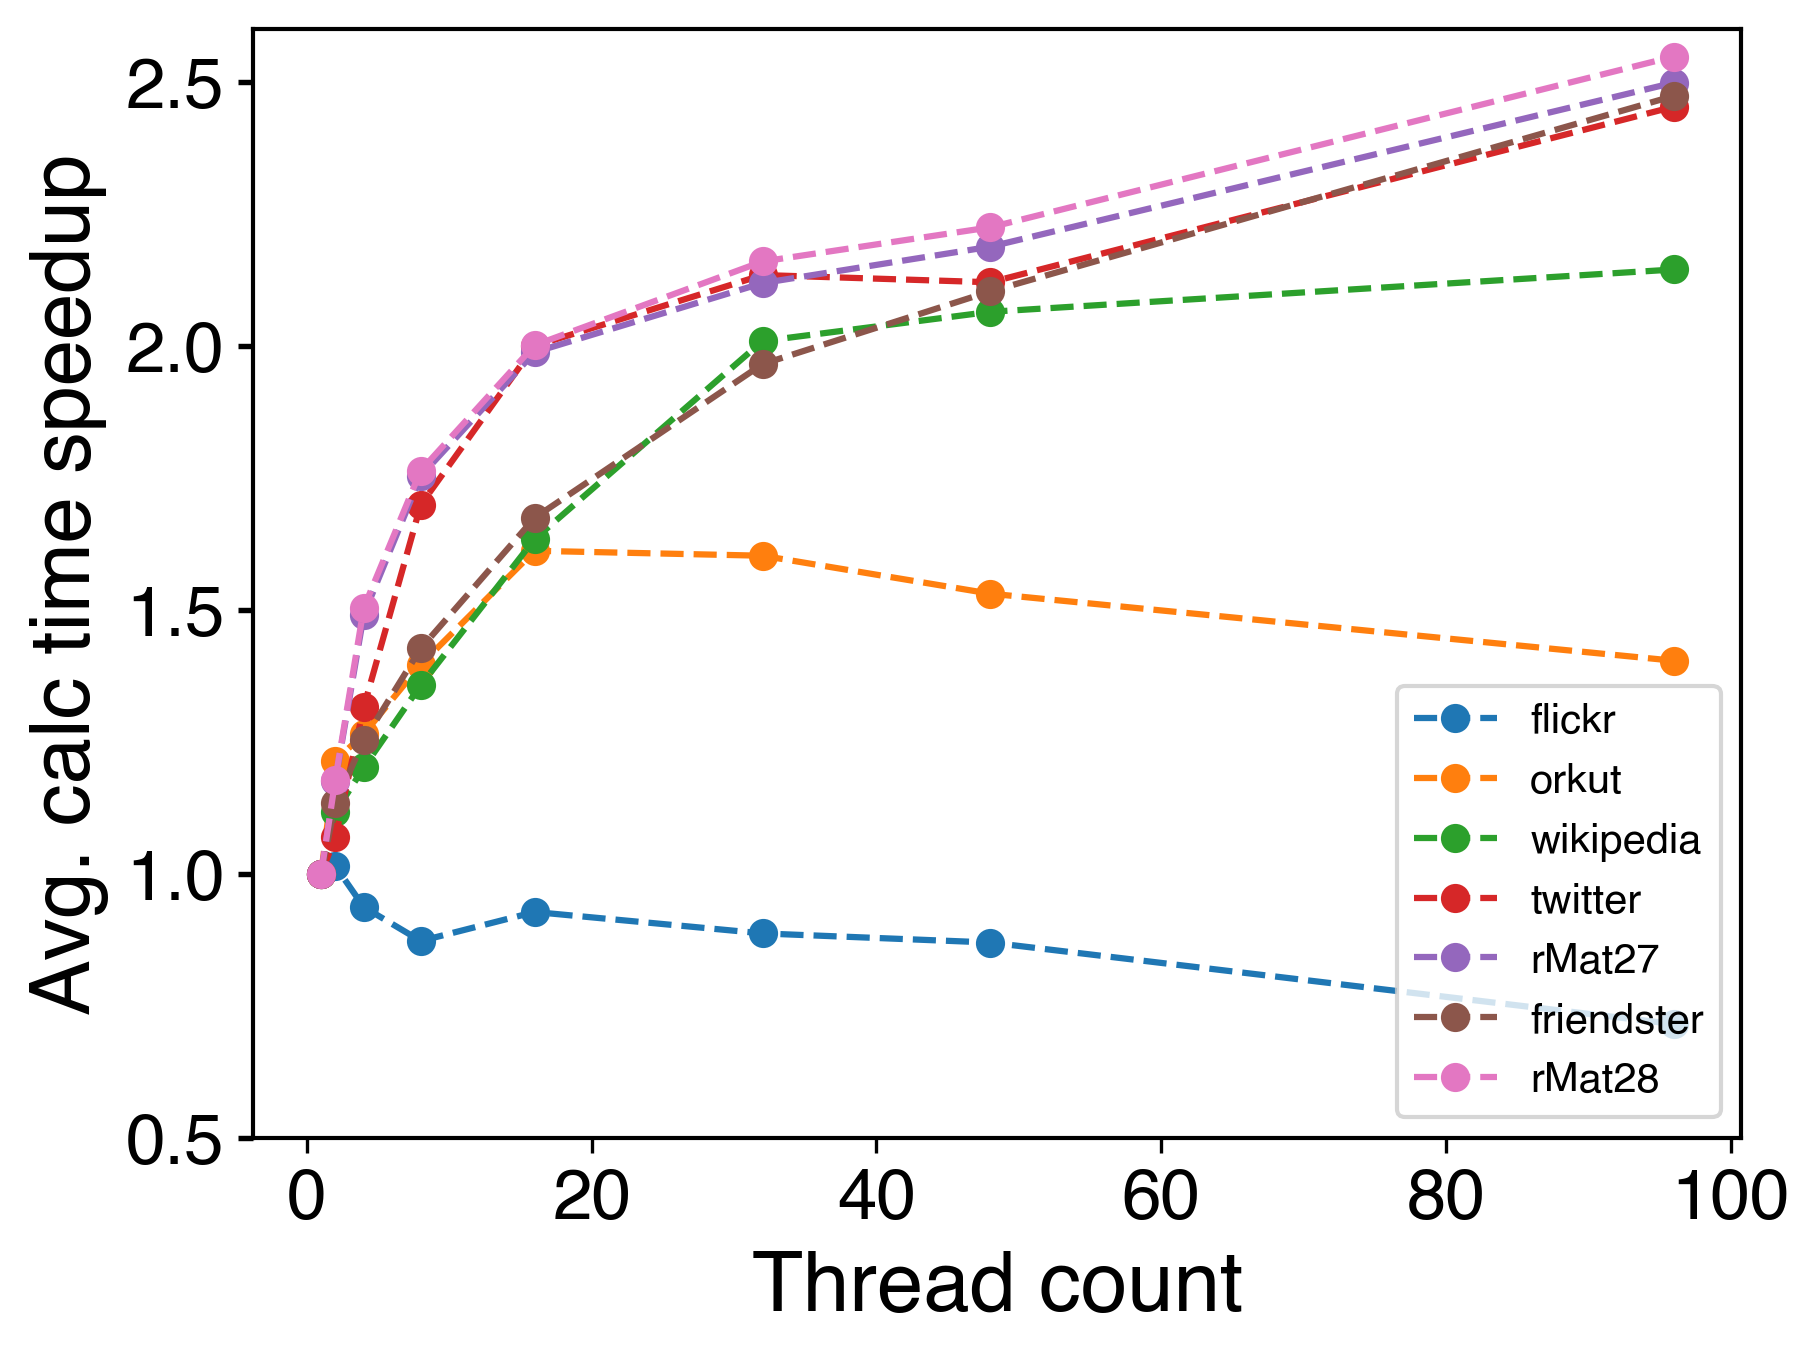
\includegraphics[width=\linewidth]{../../plots/singleNodePRPullGaloisHPThreads.png}
		\caption{PageRank Pull}
		\label{fig:galoisHPSpeedupPRPull}
	\end{subfigure}
	\begin{subfigure}{\columnwidth}
		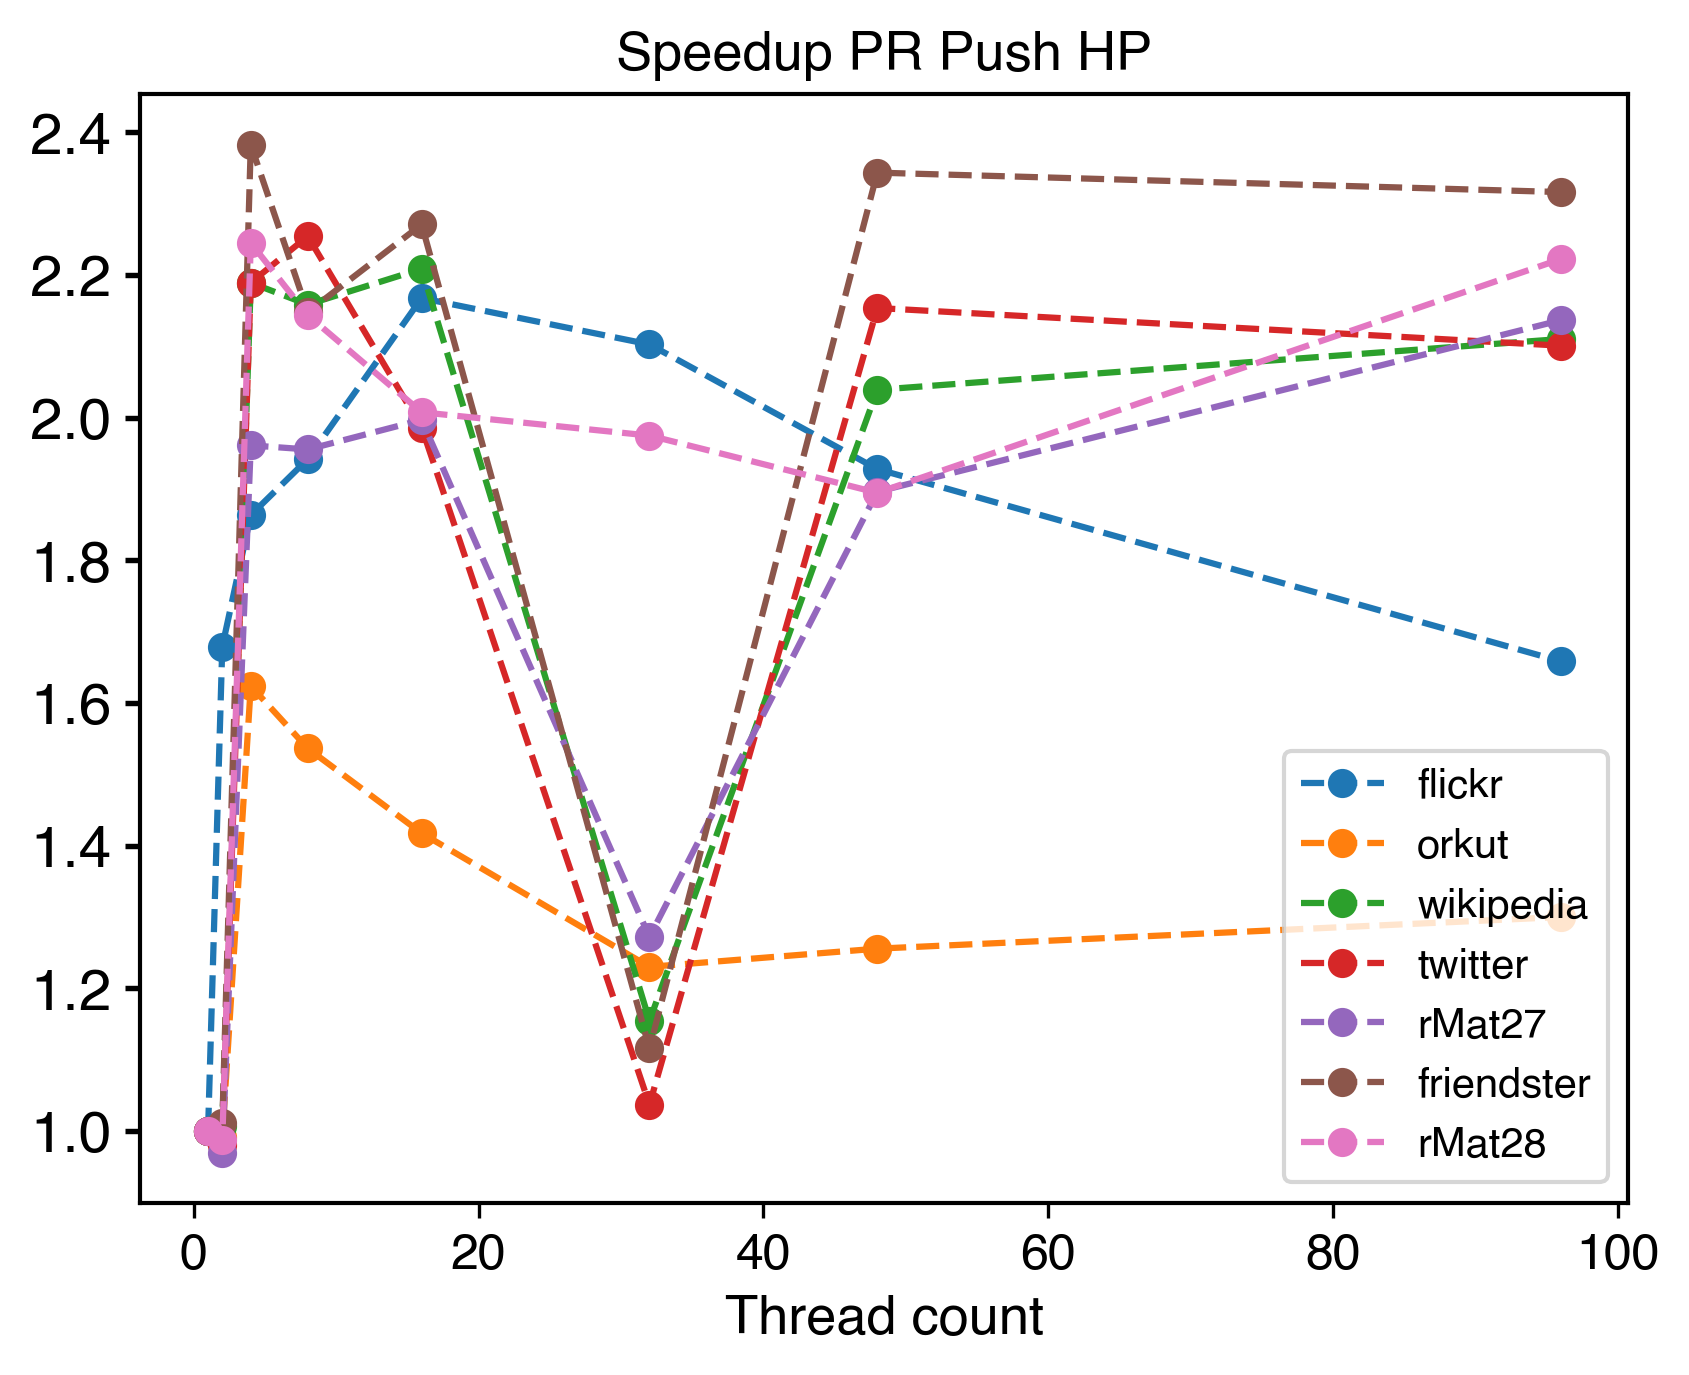
\includegraphics[width=\linewidth]{../../plots/singleNodePRPushGaloisHPThreads.png}
		\caption{PageRank Push}
		\label{fig:galoisHPSpeedupPRPush}
	\end{subfigure}
	\caption{Calculation time speedup with increasing thread count for Galois PageRank Push and Pull algorithms using Hugepages.}
\end{figure}






% \begin{figure}
% 	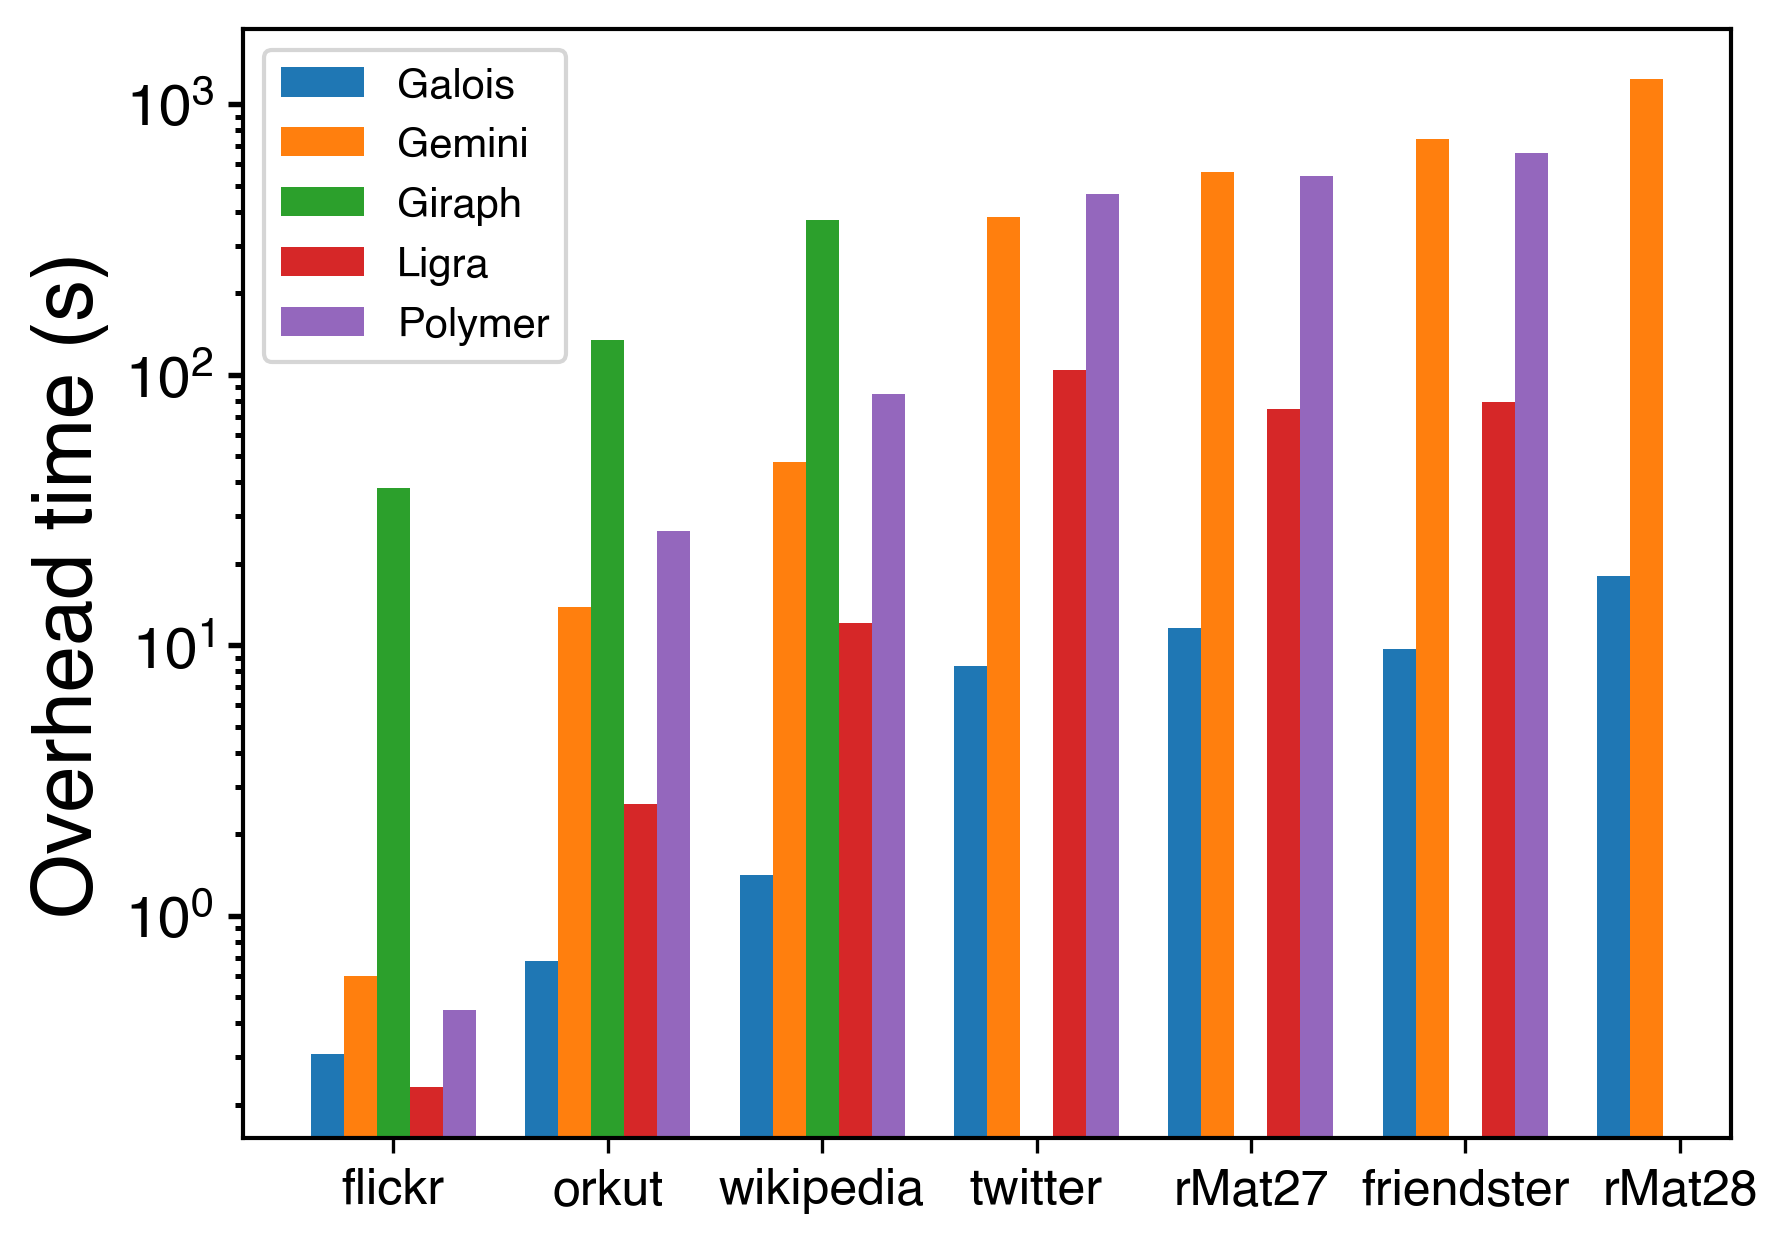
\includegraphics[width=\columnwidth]{../../plots/singleNodeSSSP_overheadTime.png}
% 	\caption{Overhead SSSP single node}
% 	\label{fig:singleNodeSSSP_overhead}
% \end{figure}



% \begin{figure}
% 	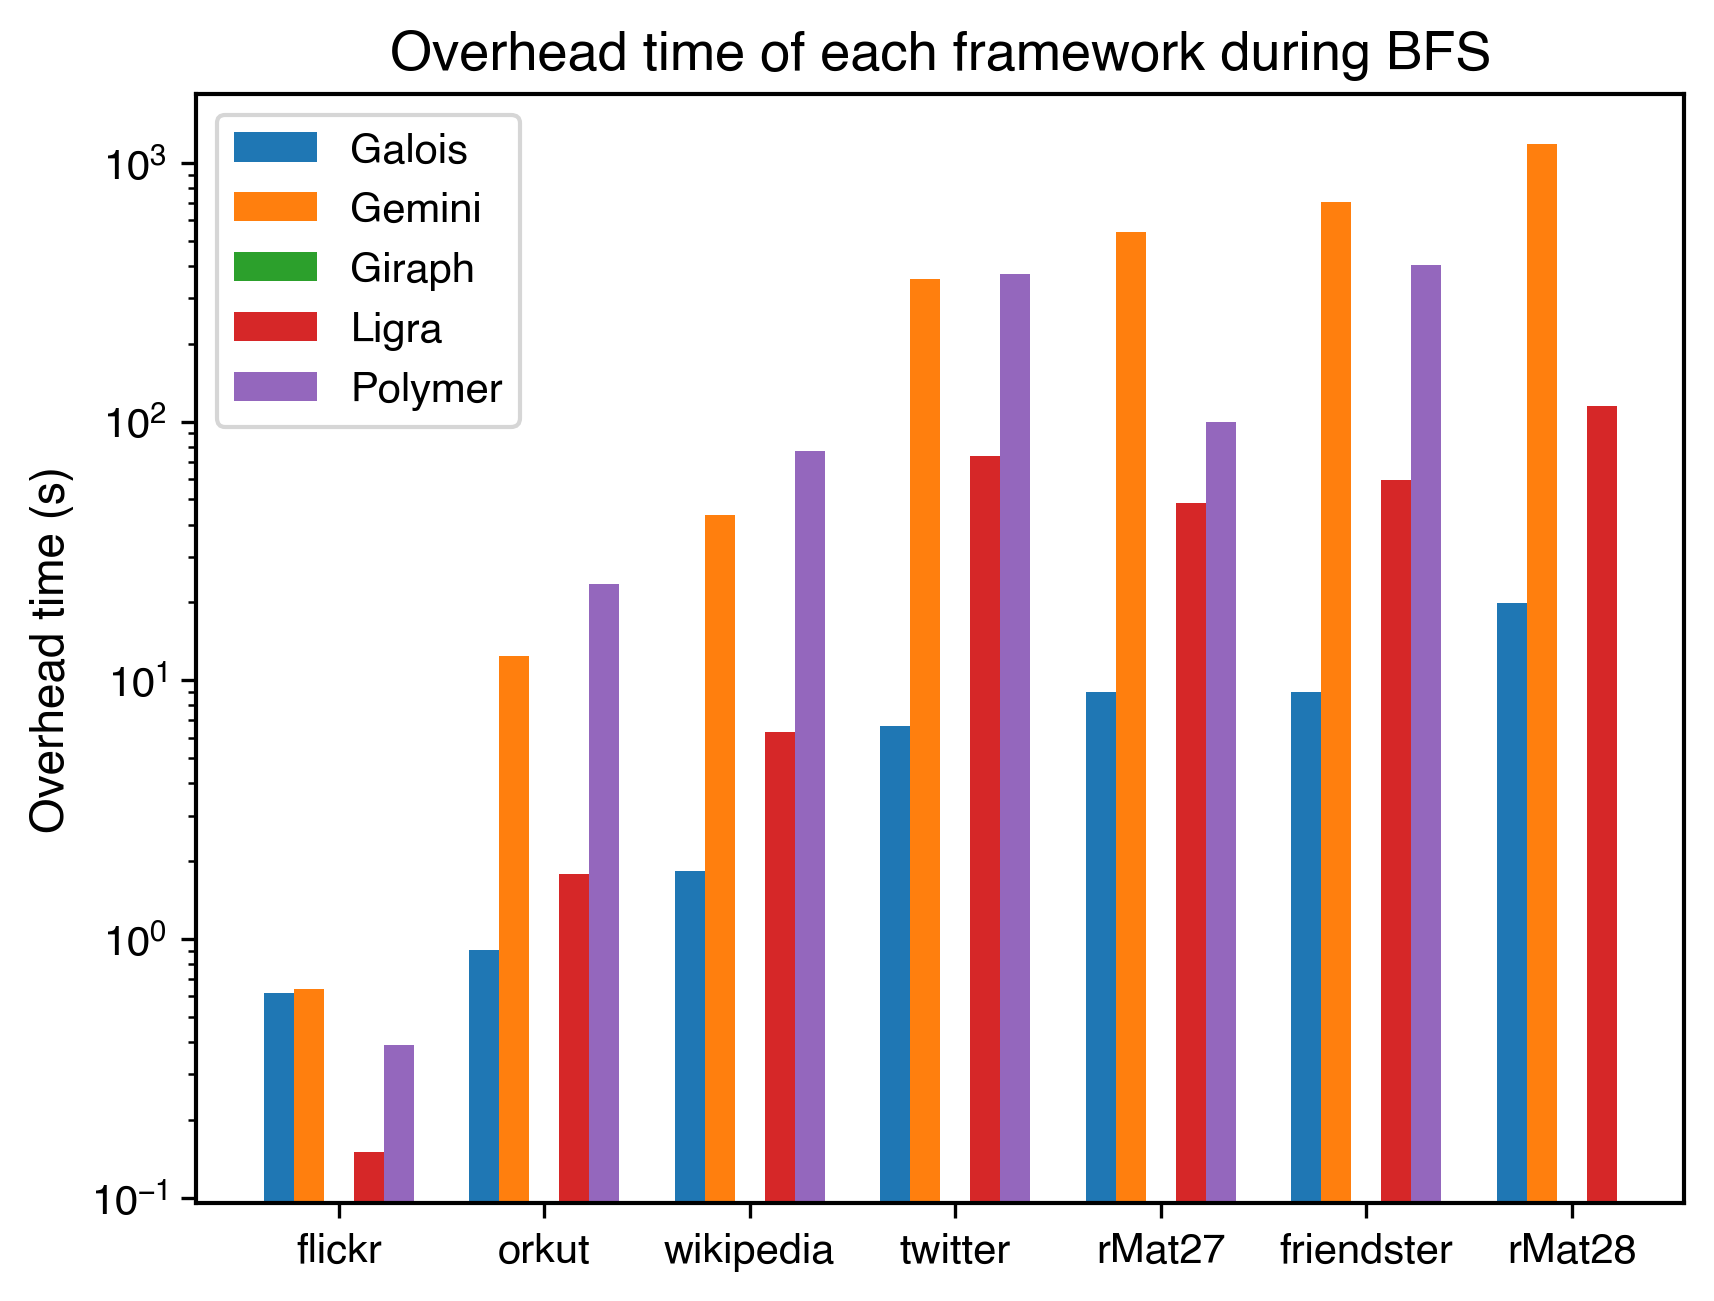
\includegraphics[width=\columnwidth]{../../plots/singleNodeBFS_overheadTime.png}
% 	\caption{Overhead BFS single node}
% 	\label{fig:singleNodeBFS_overhead}
% \end{figure}

